%% Template para dissertacao/tese na classe UFBAthesis
%% versao 1.0
%% (c) 2005 Paulo G. S. Fonseca
%% (c) 2012 Antonio Terceiro
%% (c) 2014 Christina von Flach
%% www.dcc.ufba.br/~flach/ufbathesis

%% Carrega a classe ufbathesis
%% Opcoes: * Idiomas
%%           pt   - portugues (padrao)
%%           en   - ingles
%%         * Tipo do Texto
%%           bsc  - para monografias de graduacao
%%           msc  - para dissertacoes de mestrado (padrao)
%%           qual - exame de qualificacao de mestrado
%%           prop - exame de qualificacao de doutorado
%%           phd  - para teses de doutorado
%%         * Media
%%           scr  - para versao eletronica (PDF) / consulte o guia do usuario
%%         * Estilo
%%           classic - estilo original a la TAOCP (deprecated) - apesar de deprecated, manter esse.
%%           std     - novo estilo a la CUP (padrao)
%%         * Paginacao
%%           oneside - para impressao em face unica
%%           twoside - para impressao em frente e verso (padrao)

% Atenção: Manter 'classic' na declaracao abaixo:
\documentclass[qual, classic, a4paper]{ufbathesis}

%% Preambulo:
\usepackage[utf8]{inputenc}

%\usepackage[authoryear]{natbib}
\usepackage{graphicx}
\usepackage{lipsum}
\usepackage{hyphenat}
\usepackage[usenames, dvipsnames, table]{xcolor}
\usepackage{booktabs}
\usepackage{pifont}
\usepackage{multirow}
\usepackage{listings} 
\usepackage{colortbl}
\usepackage{xfrac}
\usepackage[FIGTOPCAP]{subfigure}
\usepackage{tabularx}
\usepackage{ragged2e}
\usepackage{acronym}
\usepackage{float}
\usepackage{todonotes}
\presetkeys%
    {todonotes}%
    {inline,backgroundcolor=yellow}{}
    
\usepackage{blindtext}


% Siglas
\acrodef{AM}[AM]{{Aprendizado de Máquina}}
\acrodef{EMD}[EMD]{{Decomposição de Modo Empírico}}
\acrodef{RQA}[RQA]{{\textit{Recurrence Quantification Analysis}}}
\acrodef{FAPAR}[FAPAR] {{\textit{Fraction of Absorbed Photosynthesis Active Radiation}}}
\acrodef{DTW}[DTW] {{\textit {Dynamic  Time  Warping}}}
\acrodef{DE}[DE] {{Distância Euclidiana}}
\acrodef{EDR}[EDR]{{ \textit{ Edite  Distance  Real}}}
\acrodef{FCD}[FCD] {{\textit {Fluxo de Dados Contínuos}}}
\acrodef{DN}[DN] {{\textit {Detecção de Novidade}}}
\acrodef{CID}[CID]{{\textit{Complexity-Invariant Distance}}}
\acrodef{SLR}[SLR]{{\textit{Systematic  Literature  Review}}}
\acrodef{SANTS}[SANTS]{{\textit{Similarity Analysis on Nonstationary Time Series}}} 
\acrodef{MDDL}[MDDL]{{\textit{Mean Distance from the Diagonal Line}}}


% Universidade
\university{Universidade Federal da Bahia}

% Endereco (cidade)
\address{Salvador}

% Instituto ou Centro Academico
\institute{Instituto de Matem\'{a}tica}

% Nome da biblioteca - usado na ficha catalografica
\library{Biblioteca Reitor Mac\^{e}do Costa}

% Programa de pos-graduacao
\program{Programa de P\'{o}s-Gradua\c{c}\~{a}o em Ci\^{e}ncia da Computa\c{c}\~{a}o}

% Area de titulacao
\majorfield{Ci\^{e}ncia da Computa\c{c}\~{a}o}

% Titulo da dissertacao
\title{Aplicando redes de função de base radial para detecção de novidades em fluxos contínuos de dados}

% Data da defesa
% e.g. \date{19 de fevereiro de 2013}
\date{03 de Abril de 2019}
% e.g. \defenseyear{2013}
\defenseyear{2019}

% Autor
% e.g. \author{Jose da Silva}
\author{Ruivaldo Azevedo Lobão Neto}

% Orientador(a)
% Opcao: [f] - para orientador do sexo feminino
% e.g. \adviser[f]{Profa. Dra. Maria Santos}
\adviser{Ricardo Ara\'{u}jo Rios}

% Orientador(a)
% Opcao: [f] - para orientador do sexo feminino
% e.g. \coadviser{Prof. Dr. Pedro Pedreira}
% Comente se nao ha co-orientador
%\coadviser{Nome Completo do CO-ORIENTADOR}

%% Inicio do documento
\begin{document}

\pgcompfrontpage

%% Parte pre-textual
\frontmatter

\pgcomppresentationpage

%%%%%%%%%%%%%%%%%%%%%%%%%
% Ficha catalografica
%%%%%%%%%%%%%%%%%%%%%%%%%

%\authorcitationname{Silva, Mirlei Moura da } % e.g. Terceiro, Antonio Soares de Azevedo
%\advisercitationname{Sobrenome, Nome do ORIENTADOR} % e.g. Chavez, Christina von Flach Garcia
%\coadvisercitationname{Sobrenome, Nome do CO-ORIENTADOR} % e.g. Mendonca, Manoel Gomes de
%\catalogtype{Disserta\c{c}\~{a}o (Mestrado)} % e.g. ou ``Tese (Doutorado)''

%\catalogtopics{1. Primeira palavra-chave. 2. Segunda palavra-chave. 3. Terceira palavra-chave} % Listar palavras-chave do trabalho para a FICHA CATALOGRAFICA}, por exemplo, ``1. Complexidade Estrutural. 2. Qualidade de Software 3. Engenharia de Software''
%\catalogcdd{XXX.XX} % e.g.  XXX.XX (número nesse formato serah dado pela biblioteca)
%\catalogcdu{XXX.XX.XXX} % e.g.  XXX.XX.XXX (idem) 
%\catalogingsheet

%%%%%%%%%%%%%%%%%%%%%
% Termo de aprovacaoo
%%%%%%%%%%%%%%%%%%%%%

\approvalsheet{Salvador, 03 de Abril de 2019}{
   \comittemember{Prof. Dr. Ricardo Araújo Rios}{UFBA}  
   %\comittemember{Profa. Dr...}{UFBA}
   %\comittemember{Prof. Dr...}{USP} 
}
   % Para mestrado, apenas 3.
   % \comittemember{Prof. Dr. Professor 4}{Universidade HJKL}
   % \comittemember{Profa. Dra. Professora 5}{Universidade QWERTY}

%%%%%%%%%%%%%%%%%%%%%%%%%%%%%%%%%%%%%%%% 
% Dedicatoria, Agradecimentos, Epigrafe
%%%%%%%%%%%%%%%%%%%%%%%%%%%%%%%%%%%%%%%%

% Comente para ocultar
%\begin{dedicatory}
%DIGITE A DEDICATORIA AQUI
%\end{dedicatory}

% Agradecimentos
% Se preferir, crie um arquivo `a parte e o inclua via \include{}
%\acknowledgements
%DIGITE OS AGRADECIMENTOS AQUI

% Epigrafe
%\begin{epigraph}[NOTA]{AUTOR}
%DIGITE AQUI A CITACAO
%\end{epigraph}

%%%%%%%%%%%%%%%%%%%%%
% Resumo 
%%%%%%%%%%%%%%%%%%%%%
\resumo

\blindtext

% Palavras-chave do resumo em Portugues
\begin{keywords}
    Aprendizado de Máquina, Fluxos Contínuos de Dados, Mudanças de Conceito, Redes de Função de Base Radial, Não supervisionado
\end{keywords}

\abstract

\blindtext

% Palavras-chave do resumo em Ingles
\begin{keywords}
    Machine Learning, Data Streams, Concept Drift, Radial Basis Function Networks, Unlabeled
\end{keywords}

%%%%%%%%%%%%%%%%%%%
% Sumario / Indice
%%%%%%%%%%%%%%%%%%%

% Comente para ocultar
\tableofcontents

% Lista de figuras
% Comente para ocultar
\listoffigures

% Lista de tabelas
% Comente para ocultar
\listoftables

%% Parte textual
\mainmatter

% Eh aconselhavel criar cada capitulo em um arquivo separado, digamos
% "capitulo1.tex", "capitulo2.tex", ... "capituloN.tex" e depois
% inclui-los com:
% \include{capitulo1}
% \include{capitulo2}
% ...
% \include{capituloN}
%
% Importante: 
% Use \xchapter{}{} ao inves de \chapter{}; se não quiser colocar texto antes do inicio do capitulo, use \xchapter{texto}{}.

%%%
\xchapter{Introdução}{} \label{introducao}

\section{Contexto e Motivação}

A quantidade de dados produzidos por sistemas computacionais tem crescido exponencialmente.
Relatório do IDC (\textit{International Data Corporation}) estimava que em 2014 seriam produzidos 4,4 zettabytes (trilhões de gigabytes) de dados \cite{idc_report}.
O mesma relatório, prevê que em 2020 essa quantidade será de 44 zettabytes.

Grande parte desses sistemas produz dados através de sequências de eventos.
Estas sequências são geradas de forma contínua, ordenada, em alta frequência e potencialmente infinita \cite{Feigenbaum:2003:ALD:589343.592594}.
Na literatura, sequências com essas características são denominadas Fluxos Contínuos de Dados (FCDs).
Exemplos de sistemas que produzem fluxos dessa natureza, incluem:
monitoramento de dados de sensores \cite{Lee:Wang:Ryu:2007},
tráfico TCP/IP, 
histórico de compra de clientes,
filtragem de SPAM em mensagens de e-mail \cite{Katakis:2010:TRC:1746286.1746291},
detecção de intrusos \cite{Lane:1998:AOL:3000292.3000339},
análise de sentimentos \cite{Smailovic:2014:SAL:2941772.2941857}, 
etc.

Nos últimos anos, técnicas de Aprendizado de Máquina (AM) aplicadas a fluxos contínuos de dados têm se tornado um importante tema de pesquisa.
Nestes cenários, os algoritmos de aprendizagem devem atender a severas restrições de tempo e processamento \cite{Bifet:2009:ALM:1656274.1656287}.
Por exemplo, um classificador deve fornecer um rótulo para um evento antes que o próximo ocorra. 

Outra dificuldade encontrada nesses ambientes é a mudança na distribuição dos dados. 
Isto é, o contexto do processo gerador sofre alterações que impactam no fluxo produzido e, por conseguinte, as predições esperadas.
Este problema é conhecido como \textbf{mudança de conceito} \cite{Gama:2010:KDD:1855075} e sua ocorrência impacta a acurácia do modelo criado.
Podendo, inclusive, torná-lo obsoleto.
Estas mudanças são comumente classificadas conforme a velocidade com que ocorrem.
Mudanças de conceito \textbf{abruptas} identificam transições rápidas entre conceitos. 
Transições mais lentas, são ditas \textbf{graduais} \cite{Gama:2014:SCD:2597757.2523813}.

Como exemplificação, suponhamos que o histórico de transações via cartão de crédito de determinado cliente seja armazenado.
Este cliente, ao longo dos anos, tem utilizado o cartão apenas para comprar alimentos, sempre em uma mesma região da cidade.
A partir desse conjunto de dados, um modelo de aprendizagem é criado.
Contudo, não é coerente considerar que o comportamento do cliente permanecerá inalterado.

Diante deste contexto, devemos considerar as seguintes hipóteses:
1) Abruptamente, esse cliente compra vários eletrônicos em outro país.
Neste caso, compete aos métodos de detecção identificar se houve fraude ou se o cliente está apenas viajando e aproveitando ofertas.
2) Gradualmente, o cliente passa a utilizar o cartão para compras de passagens aéreas e diminui paulatinamente a utilização para compra de alimentos.
Após determinado período, o perfil de compra estará completamente renovado.
Assim, cabe novamente aos métodos de detecção identificar a mudança de comportamento e emitir um alerta, 
para que o modelo construído seja atualizado.

Diversos algoritmos para detecção de mudanças de conceito foram propostos na literatura.
Cada uma dessas técnicas possui características e parâmetros diferentes que visam aumentar sua eficiência, 
conforme a natureza dos dados e do tipo de mudança que se deseja otimizar.

Parte dos algoritmos detecta a mudança de conceito através do monitoramento da taxa de erro do modelo em relação a uma determinada métrica.
Alguns algoritmos que adotam essa abordagem são: 
DDM \cite{GamaMCR04}, EDDM \cite{EDDM},  
ADWIN \cite{BifetG07}, ECDD \cite{Ross:2012:EWM:2076039.2076307}, 
PL \cite{Bach:PL:2008}, FCWM \cite{FCWM}, STEPD \cite{STEPD}, DOF \cite{Sobhani:2011:NDD:2045295.2045309} e 
SCCDD/CRCDD \cite{daCosta:2016:UDS:2956219.2956389}.

Outra metodologia bastante comum para lidar com mudanças de conceito é a aplicação de comitês de classificadores (\textit{Ensemble Classifiers}). 
Esta técnica consiste na aplicação simultânea de múltiplos classificadores.
A combinação das predições individuais é utilizada para compor uma predição global \cite{Gama:2014:SCD:2597757.2523813}.
Os métodos para atualização do arranjo (criação e exclusão de classificadores) e a forma de integração das predições individuais variam para cada algoritmo.

Exemplos de comitês de classificadores são 
DWM \cite{Kolter:2007:DWM:1314498.1390333}, AUE \cite{AUE}, 
WMA \cite{Blum1997}, DDD \cite{Minku:2012:DNE:2197077.2197204}, ADOB \cite{deCarvalhoSantos:2014:SUR:3120352.3120365}, dentre outros.

As abordagens mencionadas dependem da disponibilidade do rótulo correto após determinado período de tempo.
Contudo, na maioria das aplicações reais, isto não é viável. 
Assim, foram desenvolvidos algoritmos para detecção de mudanças de conceito que não dependem dessa disponibilidade de rótulos.

Os métodos independentes de rótulos se baseiam na identificação de eventos que não se enquadram na atual estrutura dos dados \cite{Spinosa:2007:OCA:1244002.1244107}.
Técnicas de agrupamento e detecção de \textit{outliers} são comumente utilizadas nas implementações.
Além destas abordagens, estratégias de sumarização dos dados e aplicação de medidas de dissimilaridade \cite{Ryu:Kantardzic:2012} também são utilizadas para identificar novos conceitos.

Entretanto, as técnicas propostas na literatura apresentam limitações.
Algoritmos que dependem da correta rotulação são de aplicação limitada e apresentam dificuldade para lidar com mudanças abruptas.
Metodologias inspiradas em algoritmos não supervisionados envolvem maior custo computacional e tempo de resposta.
Visando resolver essas limitações, este projeto de mestrado discute um método para detecção de mudanças de conceito baseado em Redes de Função de Base Radial.

\section{Hipótese e Objetivo}

Com base nas observações citadas anteriormente, a seguinte hipótese foi formulada:

\begin{center}
\textit{``A análise de Fluxos Contínuos de Dados através de Redes de Função de Base Radial permite a detecção de mudanças de conceito, 
sem requerer a manutenção de estados prévios, de forma ágil e com precisão satisfatória em relação ao estado da arte.''}
\end{center}

O objetivo deste trabalho será o desenvolvimento e validação desta hipótese.
Para atingir este objetivo, será desenvolvido um algoritmo para detecção de mudanças de conceito baseado em Redes de Função de Base Radial. 
Este algoritmo diferencia-se por realizar a escolha dos centros de forma \textit{online}, conforme novos eventos são recepcionados, 
e por apresentar um raio dinâmico. 
A ativação de novos centros é usada como indicador para possíveis mudanças de conceito.

O algoritmo implementado será comparado com o estado da arte. 
Os fluxos utilizados nos experimentos serão divididos em dois conjuntos. 
Um conjunto formado por séries sintéticas, que permitirão uma análise detalhada da abordagem, uma vez que as características e os comportamentos dos fluxos são conhecidos. 
O outro conjunto será composto por \textit{datasets} obtidos a partir de sistemas computacionais utilizados na indústria,
visando apresentar uma aplicação prática para a solução proposta neste trabalho.


Este trabalho está organizado conforme a seguinte estrutura: 
O \textbf{Capítulo \ref{revisao_bibliografica}} possui uma revisão bibliográfica dos principais conceitos utilizados neste trabalho como, 
por exemplo, fluxos contínuos de dados, mudança de conceito e redes de função de base radial; 
No \textbf{Capítulo \ref{plano_pesquisa}} o plano de pesquisa definido é detalhado, 
identificando a metodologia que será aplicada e o cronograma de atividades. 
Por fim, o \textbf{Capítulo \ref{experimentos_iniciais}} 
apresenta um conjunto de experimentos preliminares e a análise dos resultados obtidos em relação ao estado da arte.

\xchapter{Revisão Bibliográfica}{} \label{revisao_bibliografica}
\section{Considerações Iniciais}

Este capítulo discute conceitos importantes dentro do contexto deste trabalho de pesquisa.
Em primeiro momento, Fluxos Contínuos de Dados serão descritos.
Em seguida, será abordada a ideia de Mudança de Conceito, seus tipos e características, principais algoritmos de detecção e ferramentas.
Posteriormente, serão detalhadas as Redes de Função de Base Radial.
Ao fim do capítulo, elencamos os trabalhos relacionados encontrados na literatura.


\section{Fluxos Contínuos de Dados}

Os avanços em hardware e software dos últimos anos possibilitaram a aquisição de dados em larga escala \cite{Aggarwal:2003:FCE:1315451.1315460}.
Consequentemente, tem crescido o interesse de pesquisa no gerenciamento desse grande volume de dados.
Parte relevante dessas informações é produzida através de sequências potencialmente infinitas, geradas continuamente (normalmente em alta frequência), 
conhecidas como Fluxos Contínuos de Dados (FCDs) \cite{Aggarwal:2003:FCE:1315451.1315460, Gama:2010:KDD:1855075, GamaMCR04}.
Contudo, lidar com tamanha quantidade de informações impõe desafios aos pesquisadores, sobretudo limitações de tempo de execução e recursos computacionais.

A área de Aprendizado de Máquina (AM) tem como objetivo estudar algoritmos que melhoram o seu desempenho na realização de determinada tarefa conforme ganham experiência \cite{Mitchell:1997:ML:541177}.
Atualmente, diversas técnicas de AM estão disponíveis, sendo aplicadas a uma amplo conjunto de problemas.

Segundo \cite{Gama:2010:KDD:1855075}, a área de AM dedicou-se durante muitos anos em resolver problemas de aprendizado não-incrementais (\textit{batch}), 
nos quais um conjunto de dados pré-definido é aplicado na fase de aprendizado.
Após o processamento desses dados, um modelo de decisão é gerado.
Este modelo é estático e será utilizado para realizar predições para os novos exemplos.
O cenário descrito é adequado e bastante utilizado em ambientes cuja distribuição dos dados é estacionária, 
pois o modelo preditivo permanecerá inalterado.

Contudo, os principais cenários da indústria e pesquisa que envolvem FCDs são dinâmicos.
Nestes cenários, os dados fluem de forma contínua, 
mas a distribuição que os produz pode sofrer alterações com o passar do tempo.
Isto é, são fluxos cuja distribuição dos dados não é estacionária.
Conforme \cite{Gama:Rodrigues:2009}, no contexto de classificação, o principal problema no aprendizado a partir de FCDs é a manutenção de um modelo de decisão com boa acurácia.
Para que esta continuidade seja possível, o algoritmo de aprendizado deve permitir a atualização do modelo de decisão conforme novos dados são analisados.
Esta metodologia é denominada Aprendizado Incremental \cite{Gama:2014:SCD:2597757.2523813}.

Além do aprendizado incremental, outros requisitos são necessários para aplicações de AM com FCDs.
Por receber dados de forma contínua e com intervalos curtos de tempo entre os eventos, o modelo de decisão deve produzir resultados em tempo hábil.
A quantidade de dados recebida também é muito grande, o que inviabiliza o seu armazenamento. Logo, os dados devem ser utilizados e em seguida descartados.
Além disso, com o passar do tempo, o modelo de decisão evolui, sendo necessário esquecer exemplos do passado e concentrar-se nos exemplos do presente.
Ademais, ruídos ou \textit{outliers} podem estar presentes nos dados e o algoritmo deve ser capaz de tratá-los adequadamente.
Estas são algumas das características necessárias para algoritmos de AM que lidam com FCDs, e que tornam a tarefa tão desafiadora.

Conforme \cite{Babcock:2002:MID:543613.543615} as principais diferenças de FCDs para os dados convecionais são:
\begin{itemize}
    \item Têm tamanho ilimitado;
    \item Os dados chegam de forma contínua e, geralmente, em alta velocidade;
    \item Não há controle sobre a ordem de chegada dos eventos;
    \item Processado o evento, este deve ser descartado ou armazenado, entretanto, não podendo ser recuperado facilmente.
\end{itemize}

Por serem baseados em distribuições não estacionárias, os dados evoluem ao longo do tempo.
Assim, novos conceitos (classes, grupos, etc.) podem surgir ou desaparecer, e conceitos já conhecidos podem evoluir.
Portanto, é importante que os algoritmos para FCDs consigam identificar quais dados são os mais relevantes para o contexto atual, 
quais são redundantes e quais devem ser esquecidos.

Diversas aplicações práticas da indústria e academia produzem dados em fluxos contínuos. São exemplos de aplicações:

\begin{description}
    \item[Finanças] detecção de fraudes em transações, acompanhamento da bolsa de valores;
    \item[Energia] monitoramento, predição e planejamento do consumo;
    \item[Redes e telecomunicações] monitoramento de rede, detecção de intrusos.
\end{description}

Evoluções em áreas estratégicas da computação tendem a reforçar a produção e utilização de dados produzidos através de FCDs.
Uma dessas áreas é o ramo de Internet das Coisas (\textit{Internet of Things}) \cite{iot}, 
que tem como objetivo conectar e coordenar diferentes dispositivos, sem a intervenção humana.
Pesquisa divulgada pela IDC (\textit{International Data Corporation}) prevê que serão aproximadamente 32 bilhões de dispositivos interconectados até 2020 \cite{iot}.
Portanto, algoritmos aptos a trabalhar com FCDs serão cada vez mais necessários.

\section{Mudança de Conceito}
\blindtext

\subsection{Algoritmos para Detecção de Mudança de Conceito}
\blindtext

\subsection{Ferramentas}
\blindtext

\section{Redes de Função de Base Radial}
\blindtext
  
\section{Trabalhos Relacionados}
\blindtext

\section{Considerações Finais}
\blindtext

\xchapter{Plano de Pesquisa}{} \label{plano_pesquisa}
\section{Considerações Iniciais}
\blindtext

\section{Descrição do Problema}
\blindtext

\subsection{Atividades de Pesquisa}
\blindtext

\section{Considerações Finais}
\blindtext

\xchapter{Experimentos Iniciais}{} \label{experimentos_iniciais}
\section{Considerações Iniciais}
\blindtext

\section{Configuração dos Experimentos}
\blindtext

\section{Método de Pettitt}
\blindtext

\section{Redes de Função de Base Radial}
\blindtext

\section{Considerações Finais}
\blindtext


%% Parte pos-textual
\backmatter

% Bibliografia
% É aconselhável utilizar o BibTeX a partir de um arquivo, digamos "biblio.bib".
% Para ajuda na criação do arquivo .bib e utilização do BibTeX, recorra ao
% BibTeXpress em www.cin.ufpe.br/~paguso/bibtexpress
\bibliographystyle{abntex2-alf}
\bibliography{biblio}

% Apendices
% Comente se naoo houver apendices
%\appendix

%\xchapter{Exemplo de Ap\^endice}{} %sem preambulo
%\lipsum
% Eh aconselhavel criar cada apendice em um arquivo separado, digamos
% "apendice1.tex", "apendice.tex", ... "apendiceM.tex" e depois
% inclui--los com:
%\xchapter{Decomposição das séries temporais}{} %sem preambulo
\label{apendice1}
\section{Considerações Iniciais}
Neste apêndice consta as 40 séries temporais utilizadas nos experimentos mostrados no Capitulo \ref{experimentos}. As séries foram divididas em 4 tipos conforme a Tabela \ref{series}, onde o tipo representa um conjunto de 10 séries senoide ou cossenoide, sendo acrescida de ruído ou acrescida de ruído e tendência.
Nas imagens são representadas, a séries original,   seu componente determinístico e seu componente estocástico, os quais foram extraídos após a decomposição.
\section{Séries TIPO 1}
10 séries cossenoide com ruído ao longo da série.
\graphicspath{{imagens/}}
\begin{figure}[H]
\begin{center}
  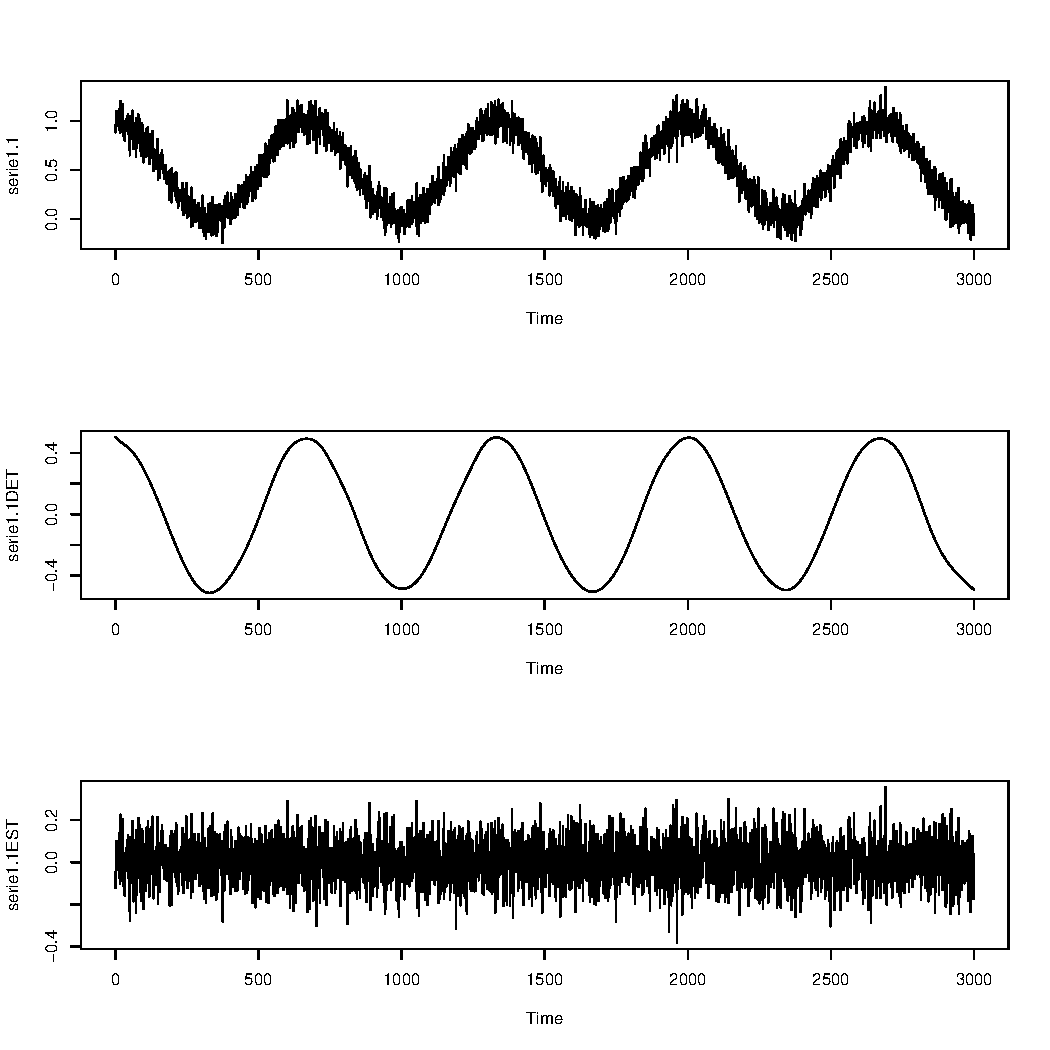
\includegraphics[scale=0.43]{serie1_1.pdf} \quad
  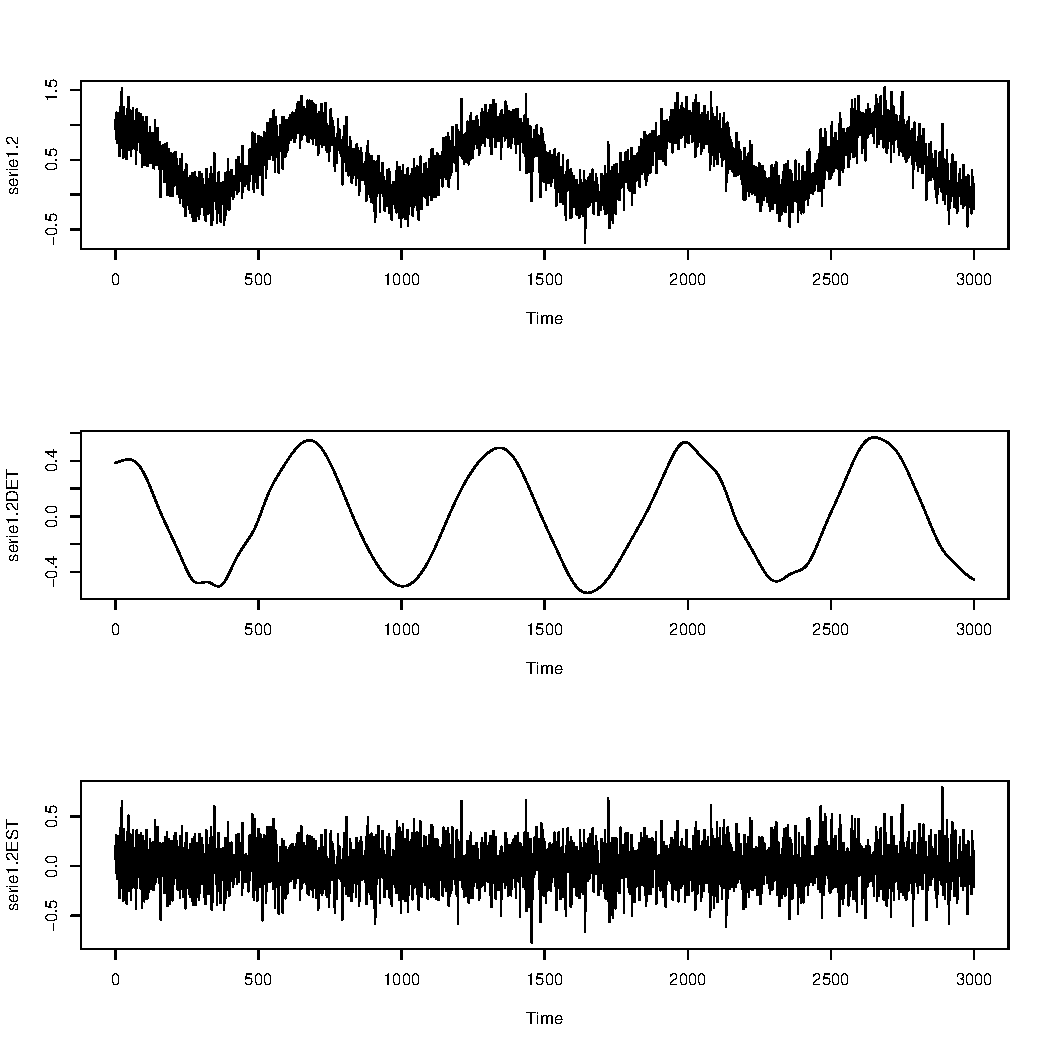
\includegraphics[scale=0.43]{serie1_2.pdf}
  \caption{Série 1.1 e Série 1.2}

\end{center}
\end{figure}

\graphicspath{{imagens/}}
\begin{figure}[H]
\begin{center}
  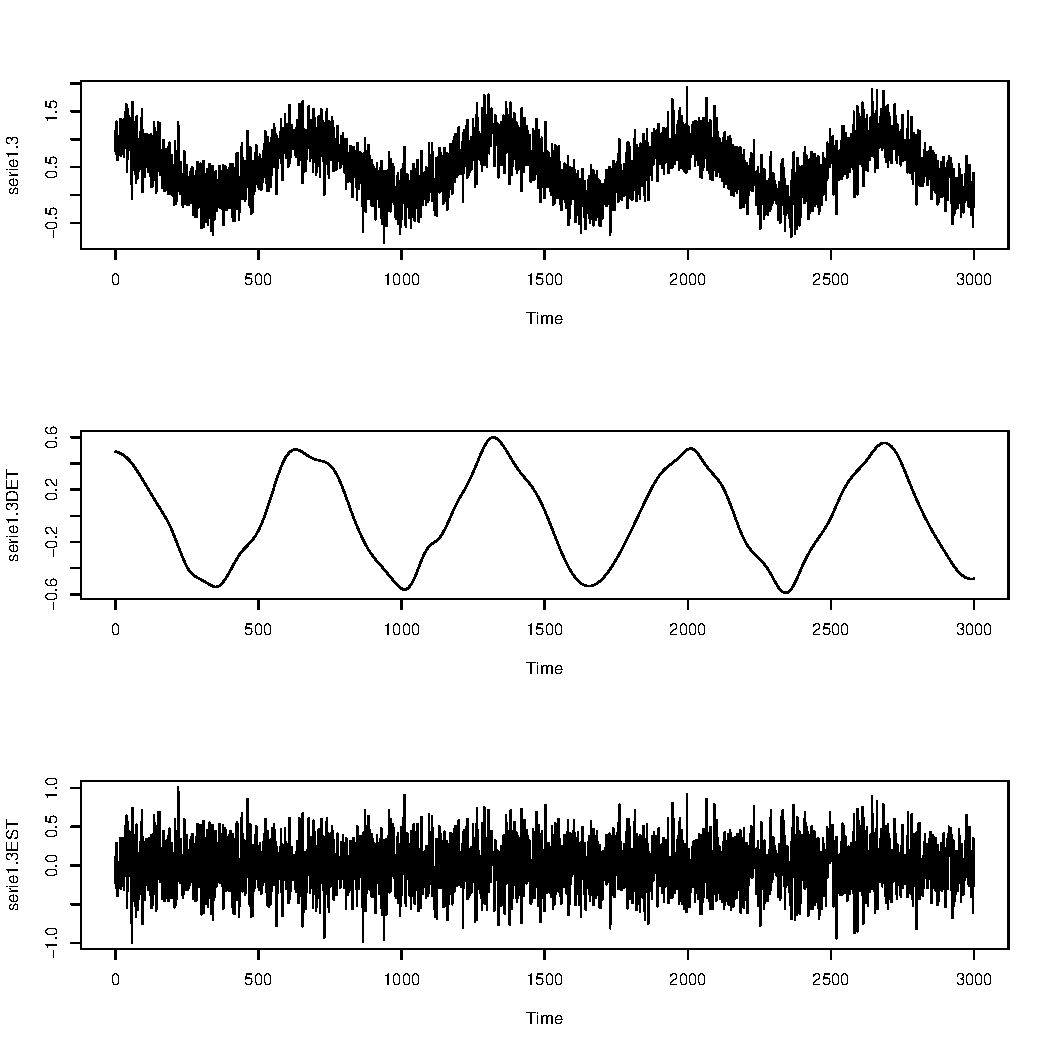
\includegraphics[scale=0.43]{serie1_3.pdf} \quad
  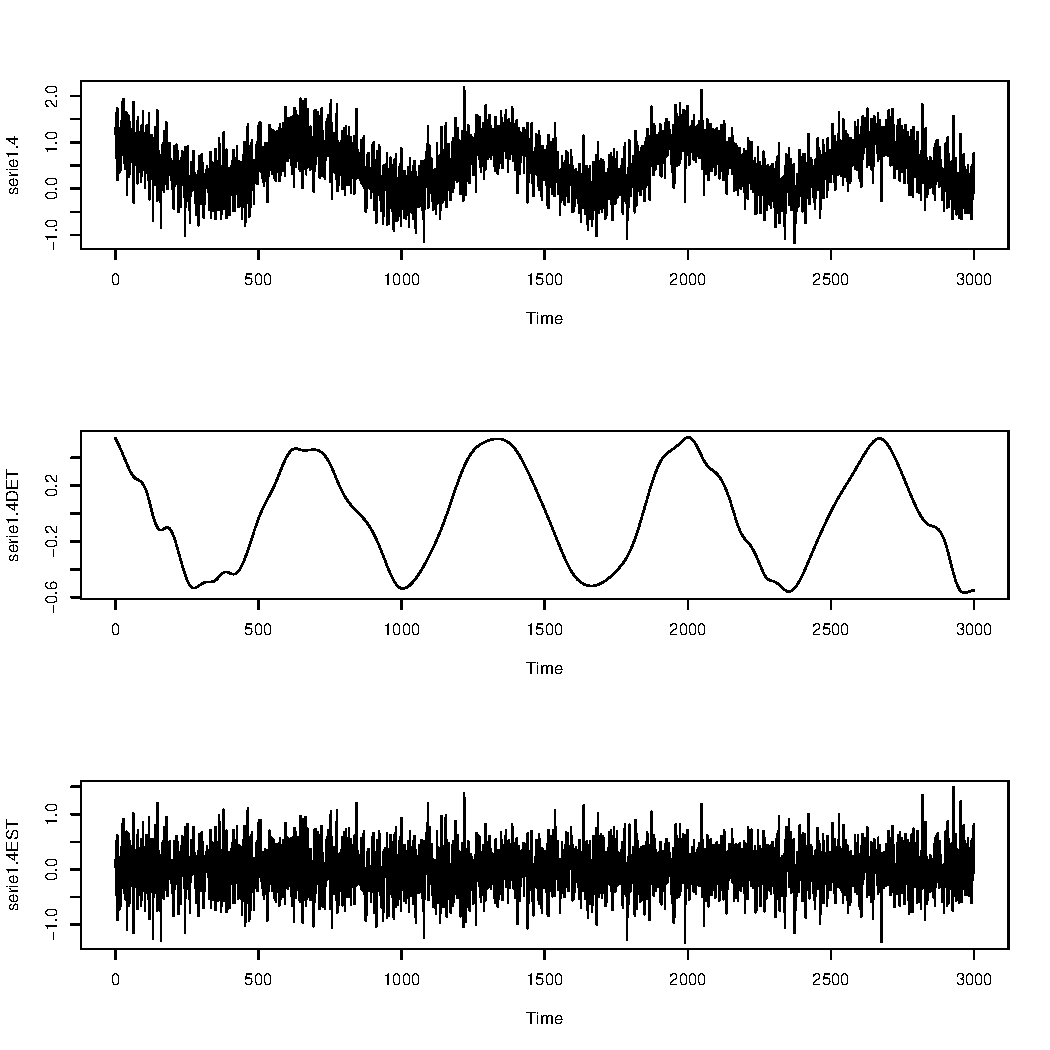
\includegraphics[scale=0.43]{serie1_4.pdf}
  \caption{Série 1.3 e Série 1.4}

\end{center}
\end{figure}

\graphicspath{{imagens/}}
\begin{figure}[H]
\begin{center}
  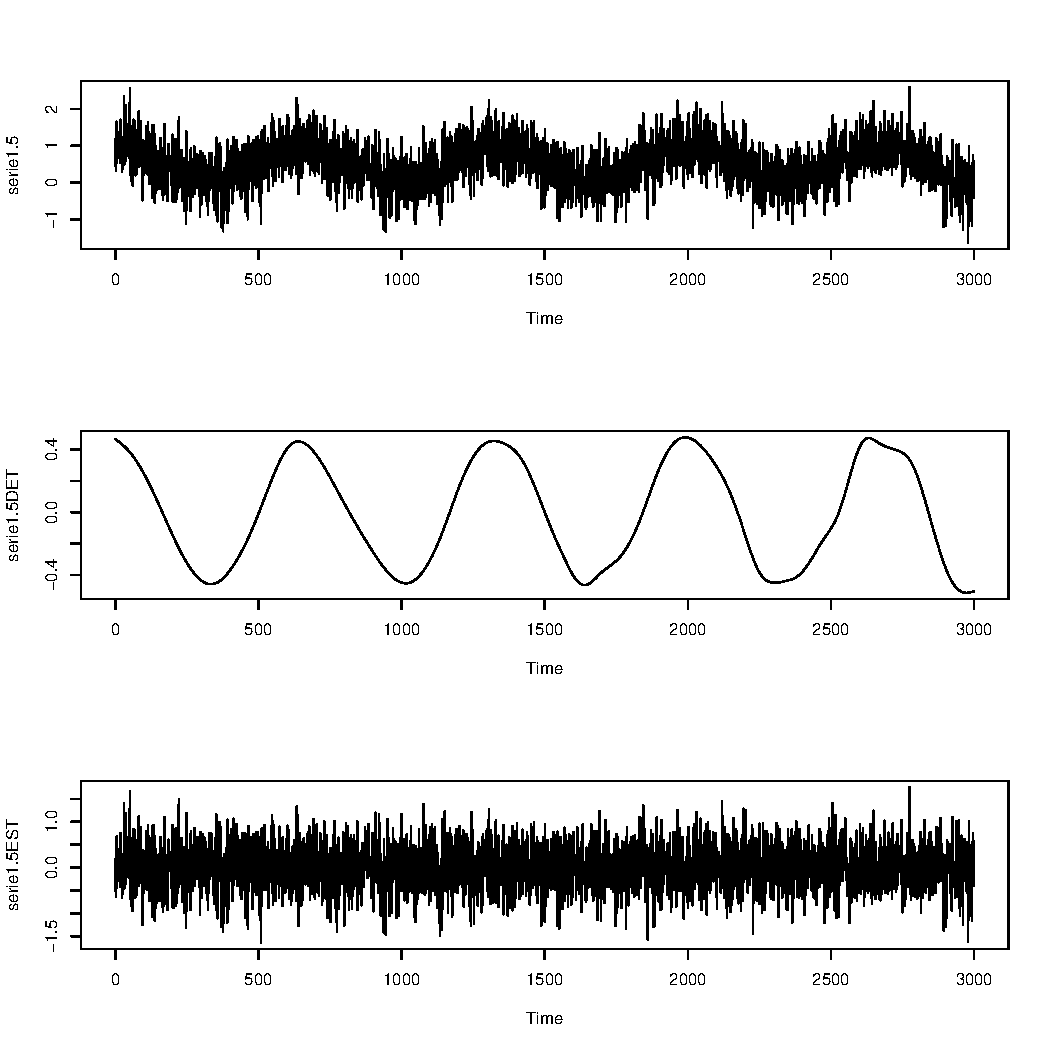
\includegraphics[scale=0.43]{serie1_5.pdf} \quad
  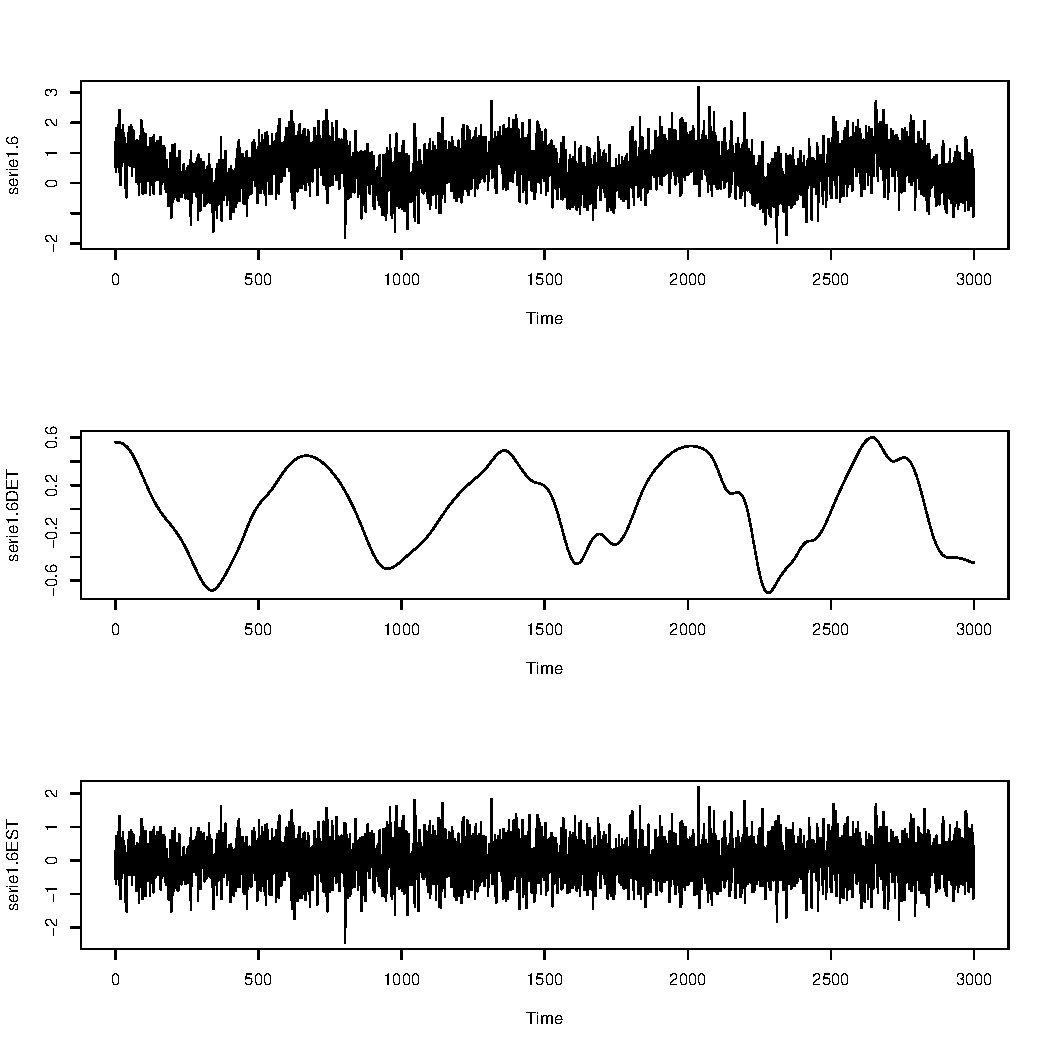
\includegraphics[scale=0.43]{serie1_6.pdf}
  \caption{Série 1.5 e Série 1.6}

\end{center}
\end{figure}

\graphicspath{{imagens/}}
\begin{figure}[H]
\begin{center}
  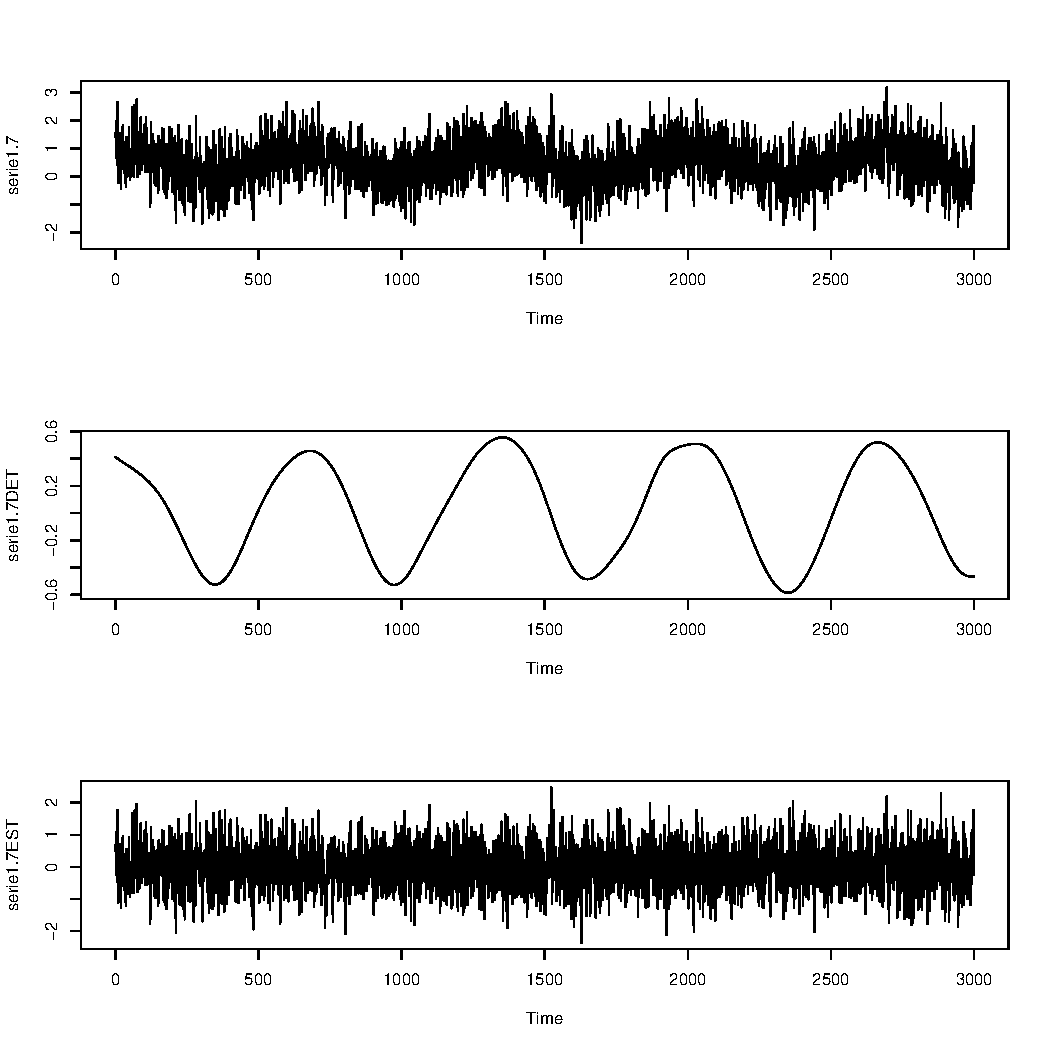
\includegraphics[scale=0.43]{serie1_7.pdf} \quad
  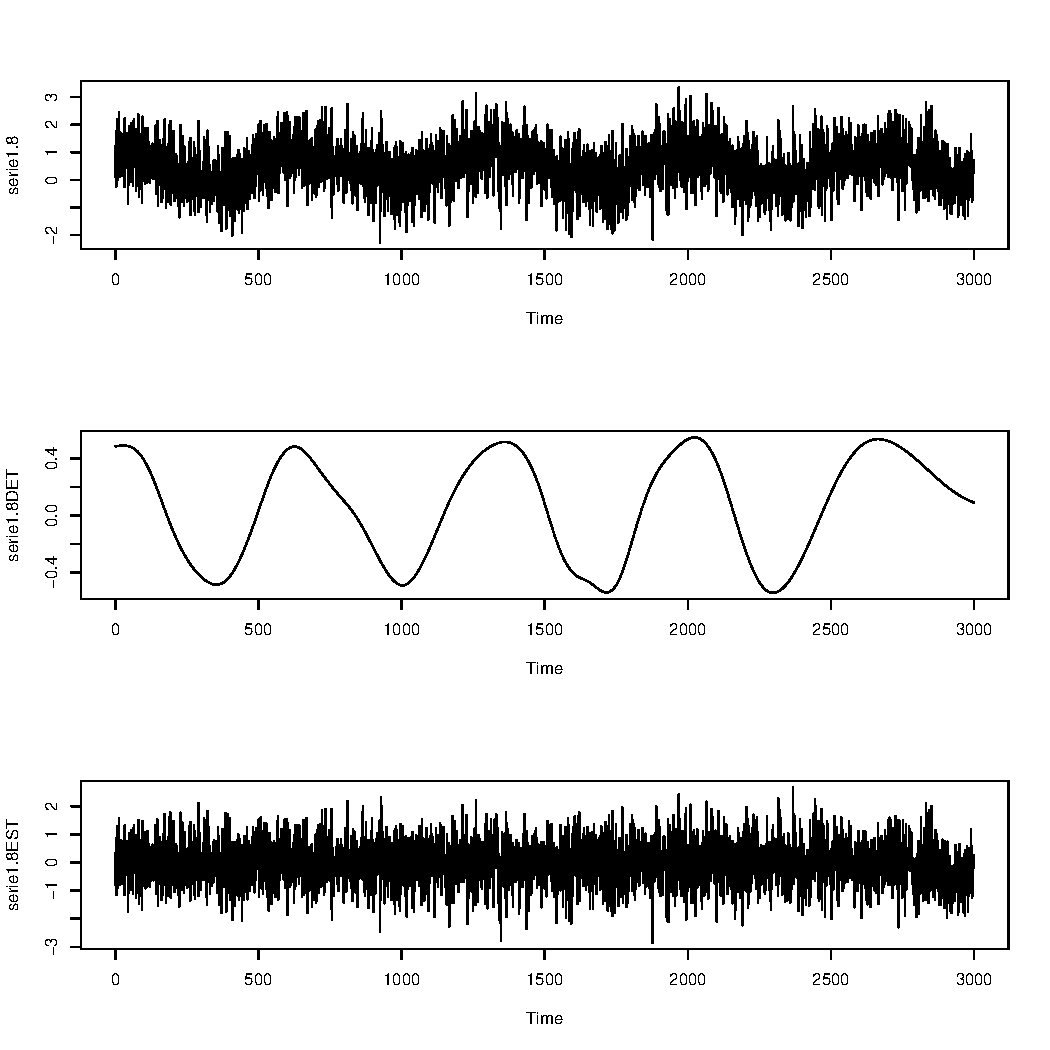
\includegraphics[scale=0.43]{serie1_8.pdf}
  \caption{Série 1.7 e Série 1.8}

\end{center}
\end{figure}

\graphicspath{{imagens/}}
\begin{figure}[H]
\begin{center}
  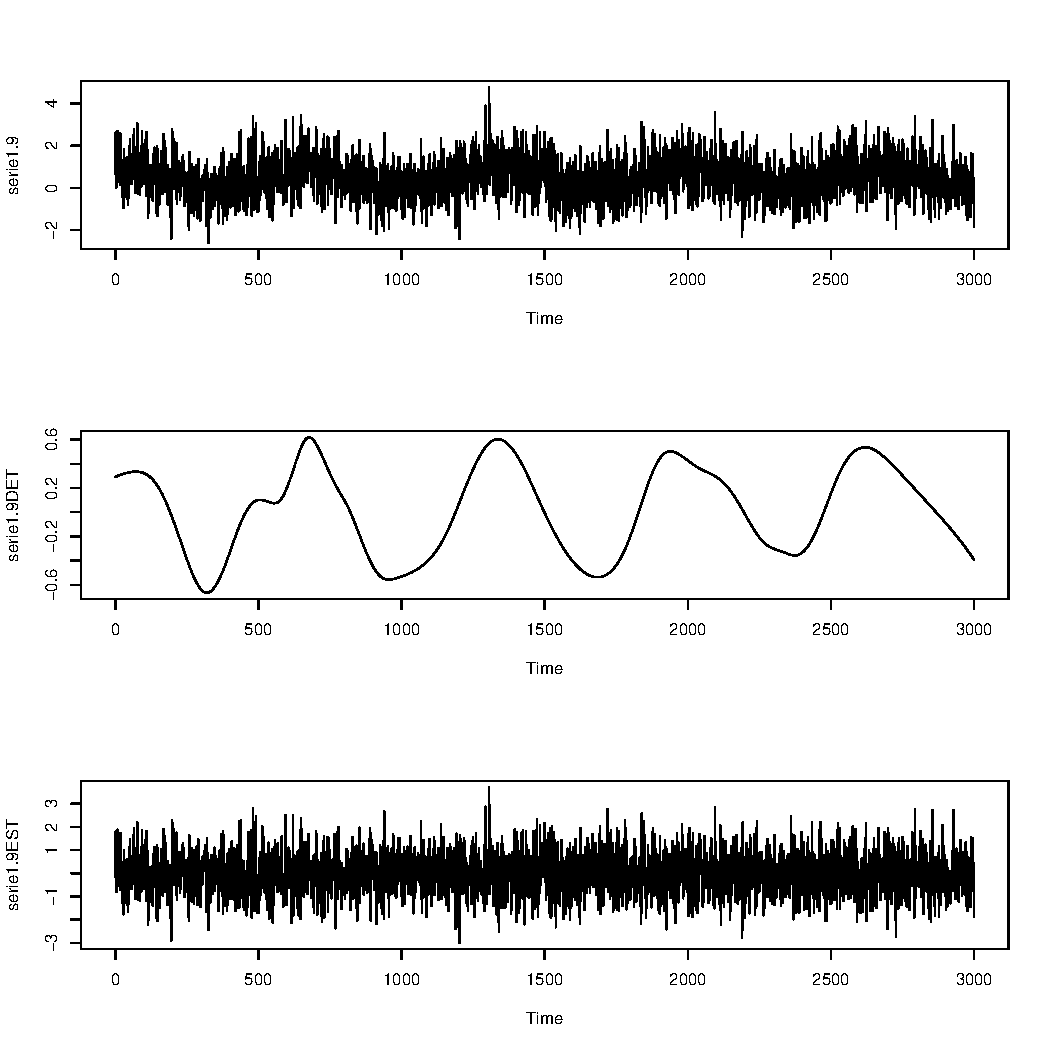
\includegraphics[scale=0.43]{serie1_9.pdf} \quad
  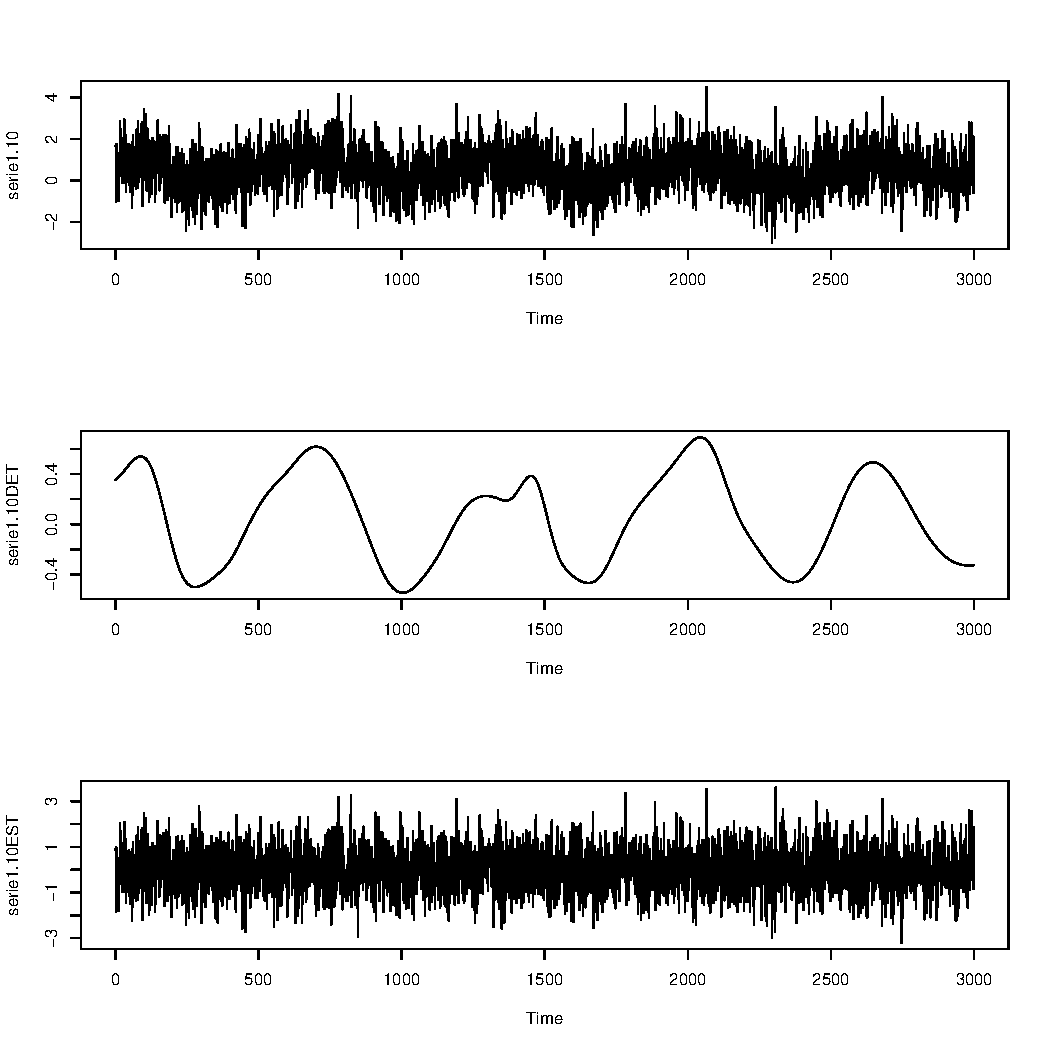
\includegraphics[scale=0.43]{serie1_10.pdf}
  \caption{Série 1.9 e Série 1.10}

\end{center}
\end{figure}

\section{Séries TIPO 2}
10 séries cossenoide com ruído ao longo da série e tendência.
\graphicspath{{imagens/}}
\begin{figure}[H]
\begin{center}
  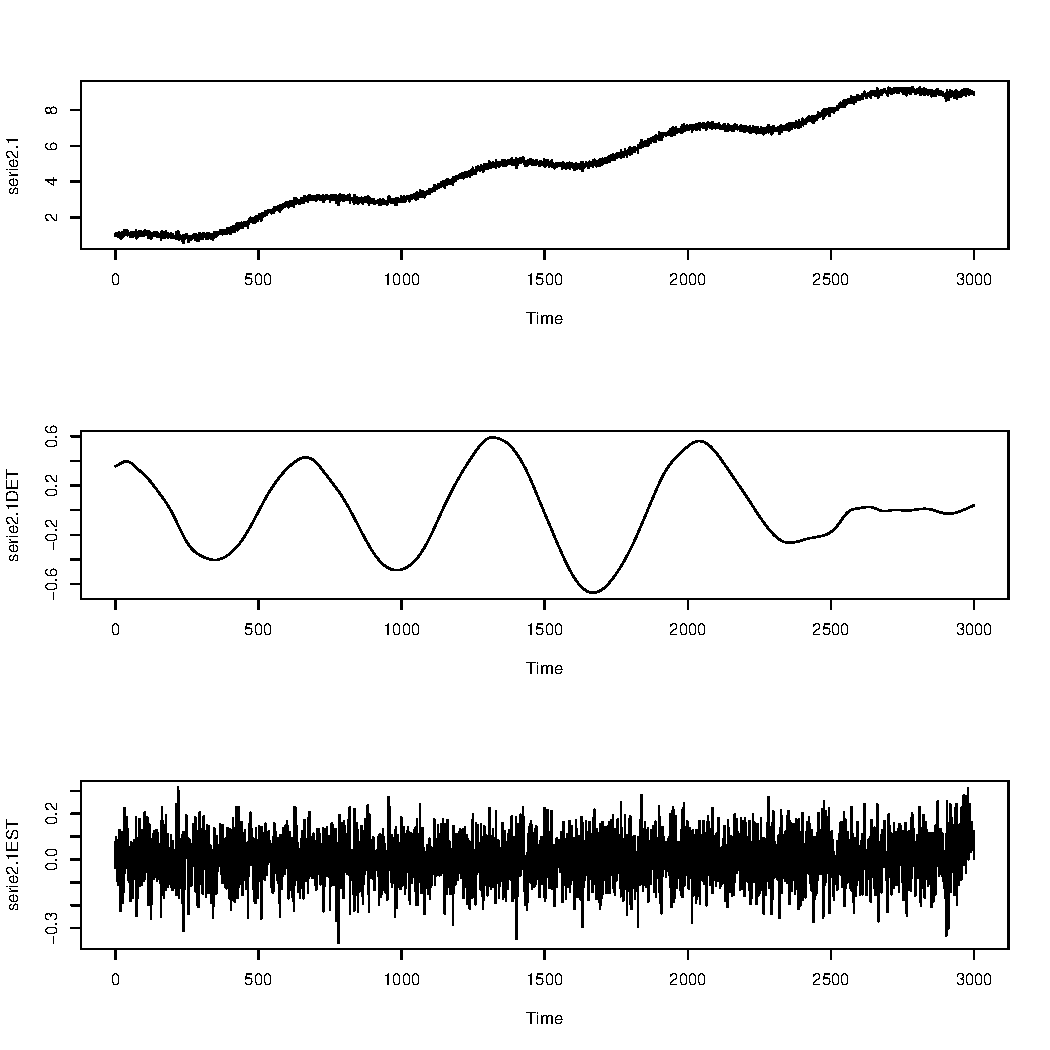
\includegraphics[scale=0.43]{serie2_1.pdf} \quad
  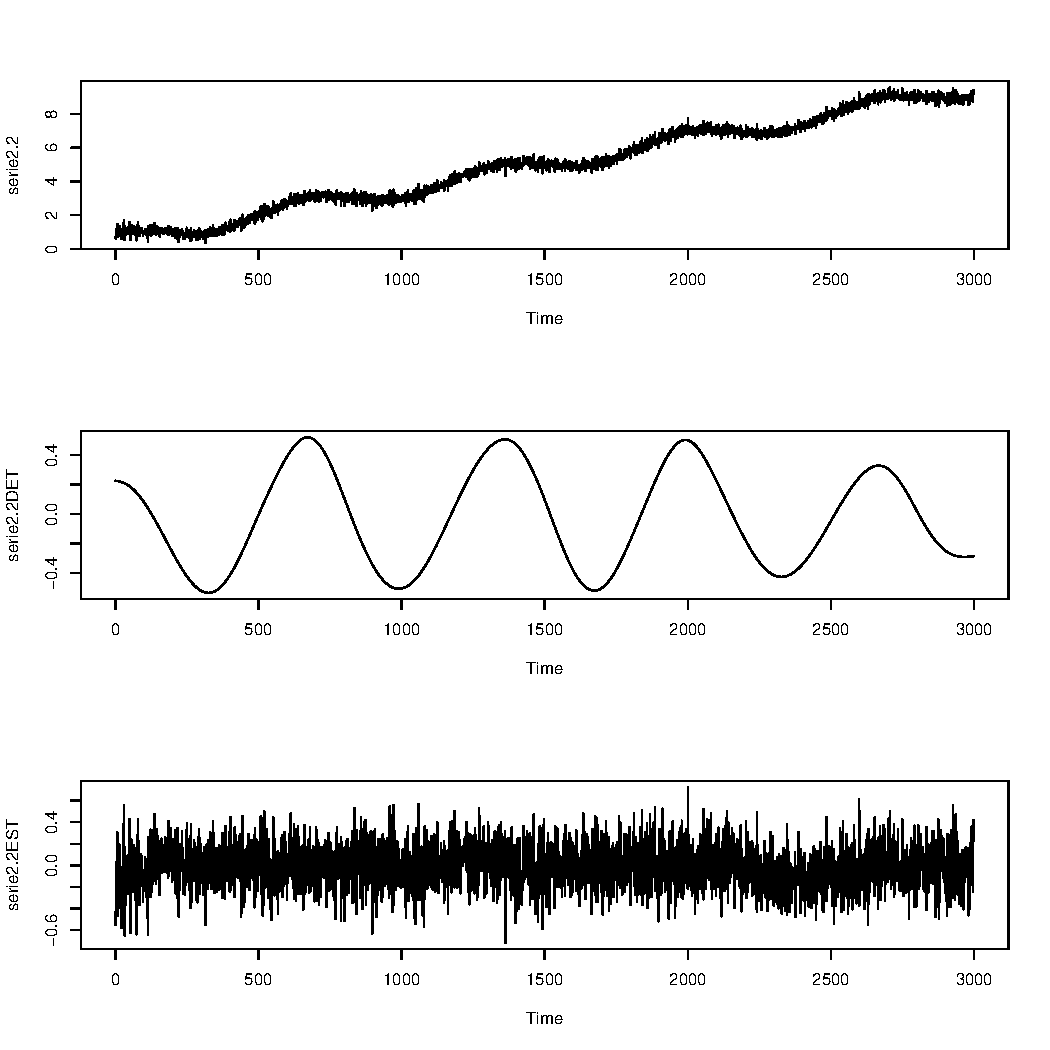
\includegraphics[scale=0.43]{serie2_2.pdf}
  \caption{Série 2.1 e Série 2.2}

\end{center}
\end{figure}

\graphicspath{{imagens/}}
\begin{figure}[H]
\begin{center}
  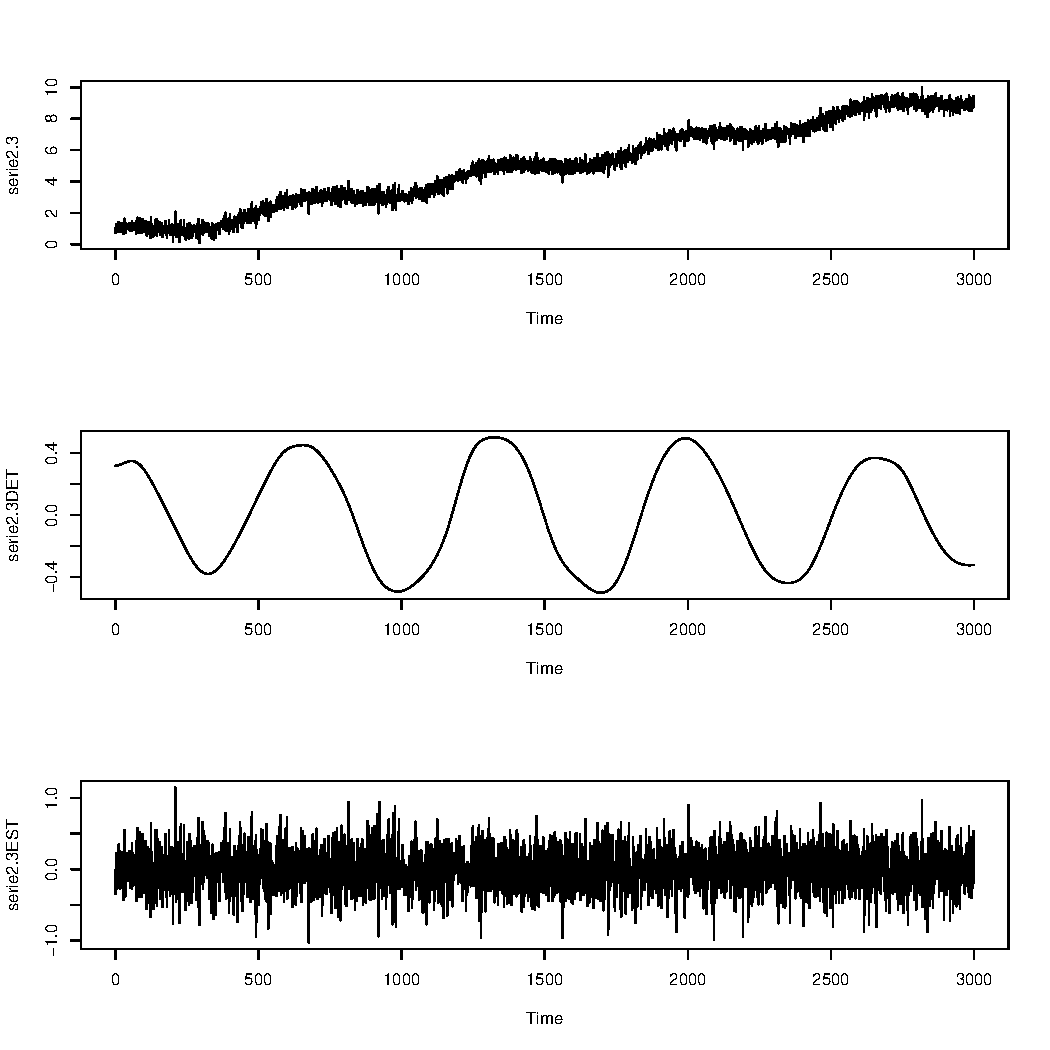
\includegraphics[scale=0.43]{serie2_3.pdf} \quad
  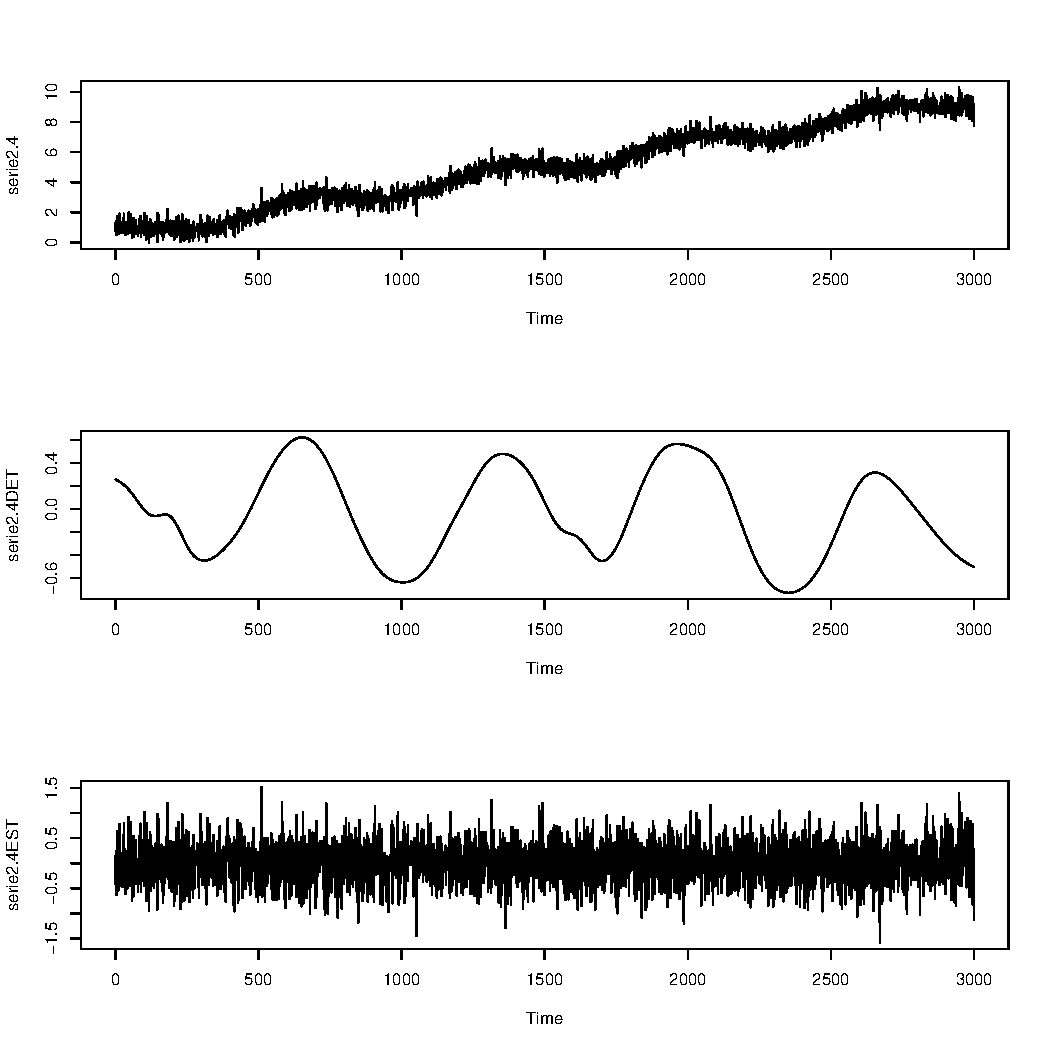
\includegraphics[scale=0.43]{serie2_4.pdf}
  \caption{Série 2.3 e Série 2.4}

\end{center}
\end{figure}

\graphicspath{{imagens/}}
\begin{figure}[H]
\begin{center}
  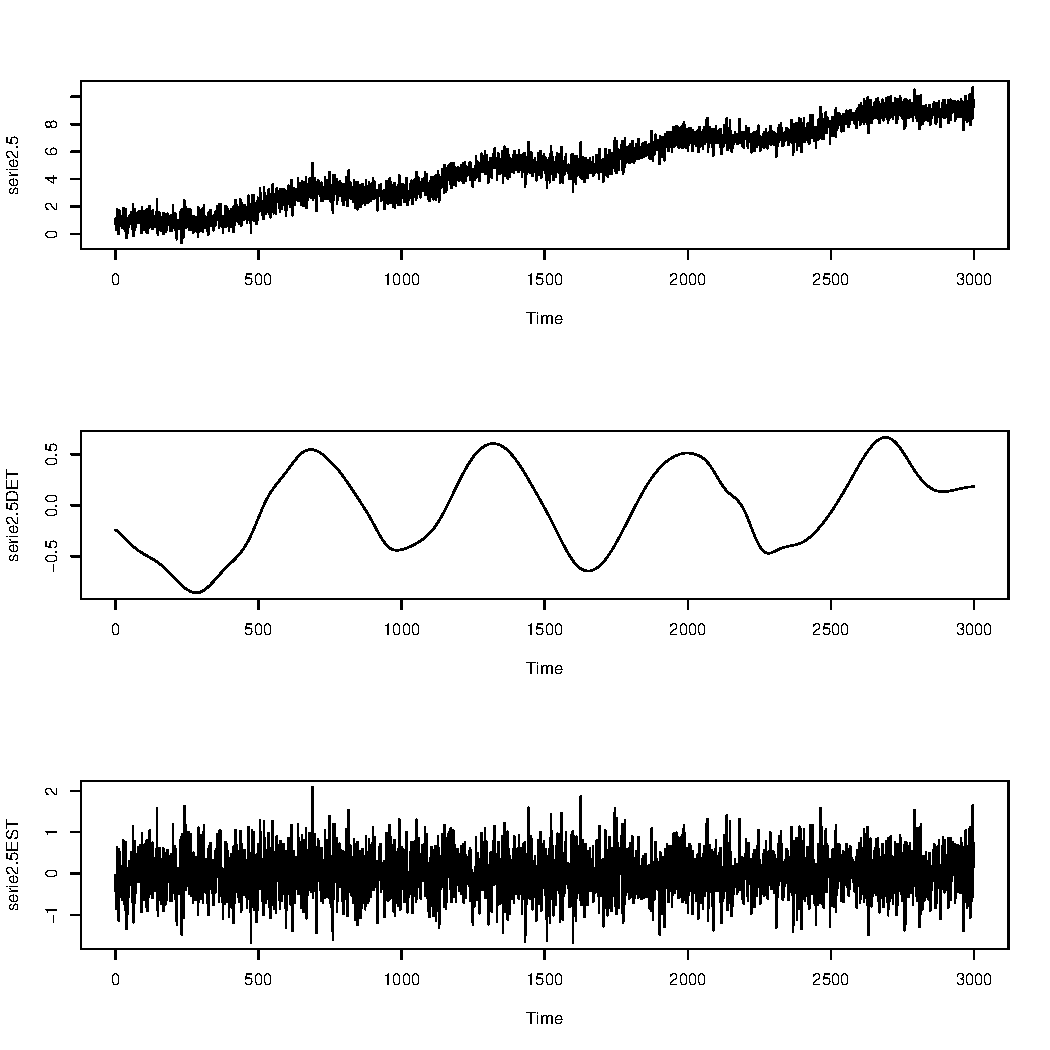
\includegraphics[scale=0.43]{serie2_5.pdf} \quad
  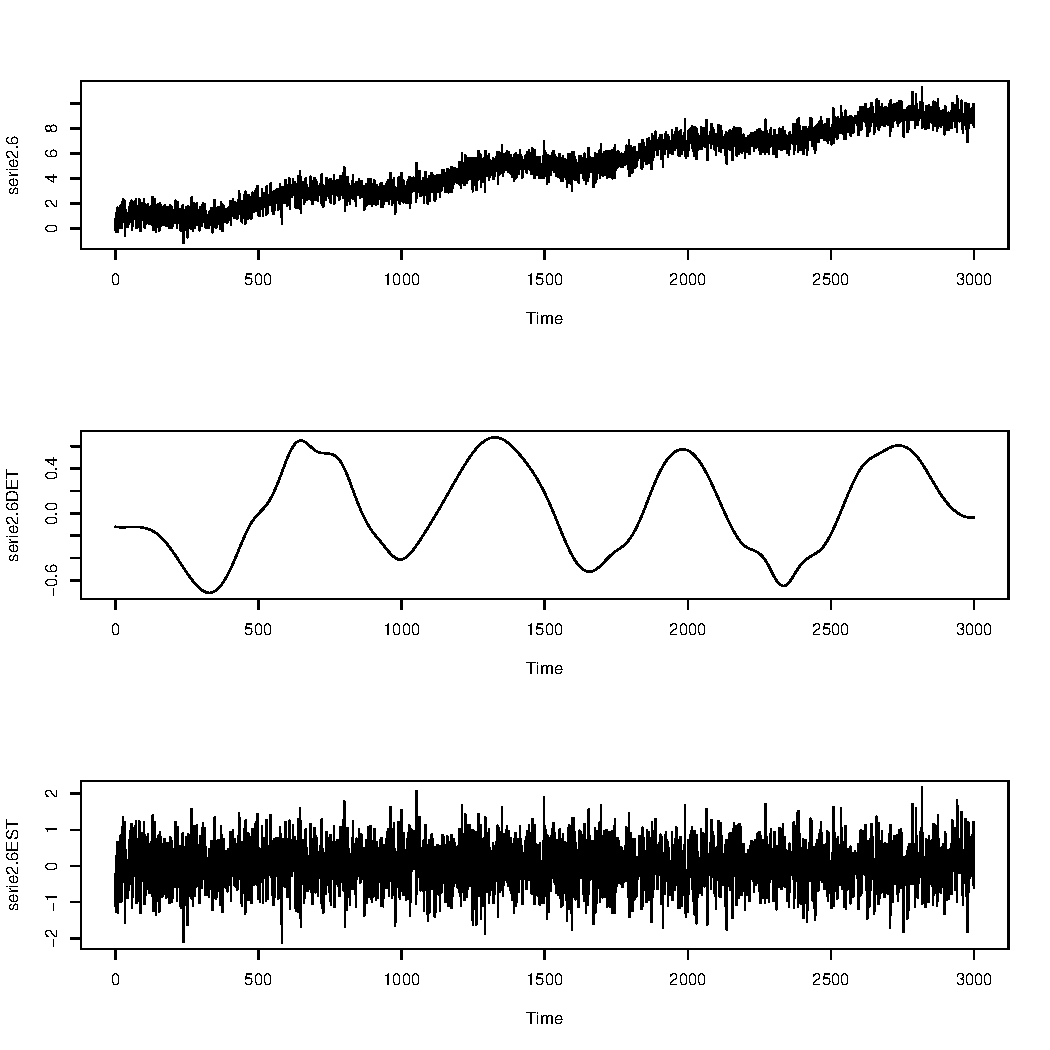
\includegraphics[scale=0.43]{serie2_6.pdf}
  \caption{Série 2.5 e Série 2.6}

\end{center}
\end{figure}

\graphicspath{{imagens/}}
\begin{figure}[H]
\begin{center}
  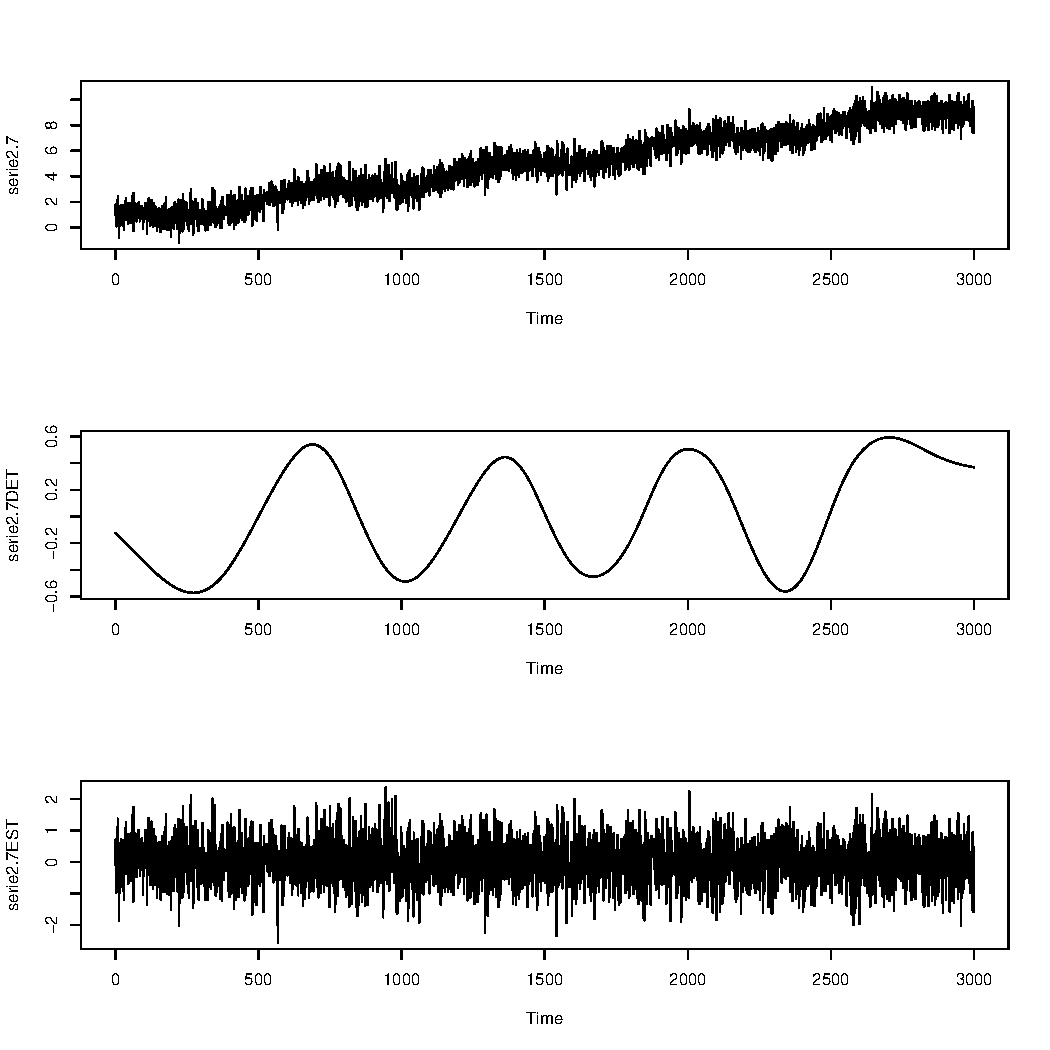
\includegraphics[scale=0.43]{serie2_7.pdf} \quad
  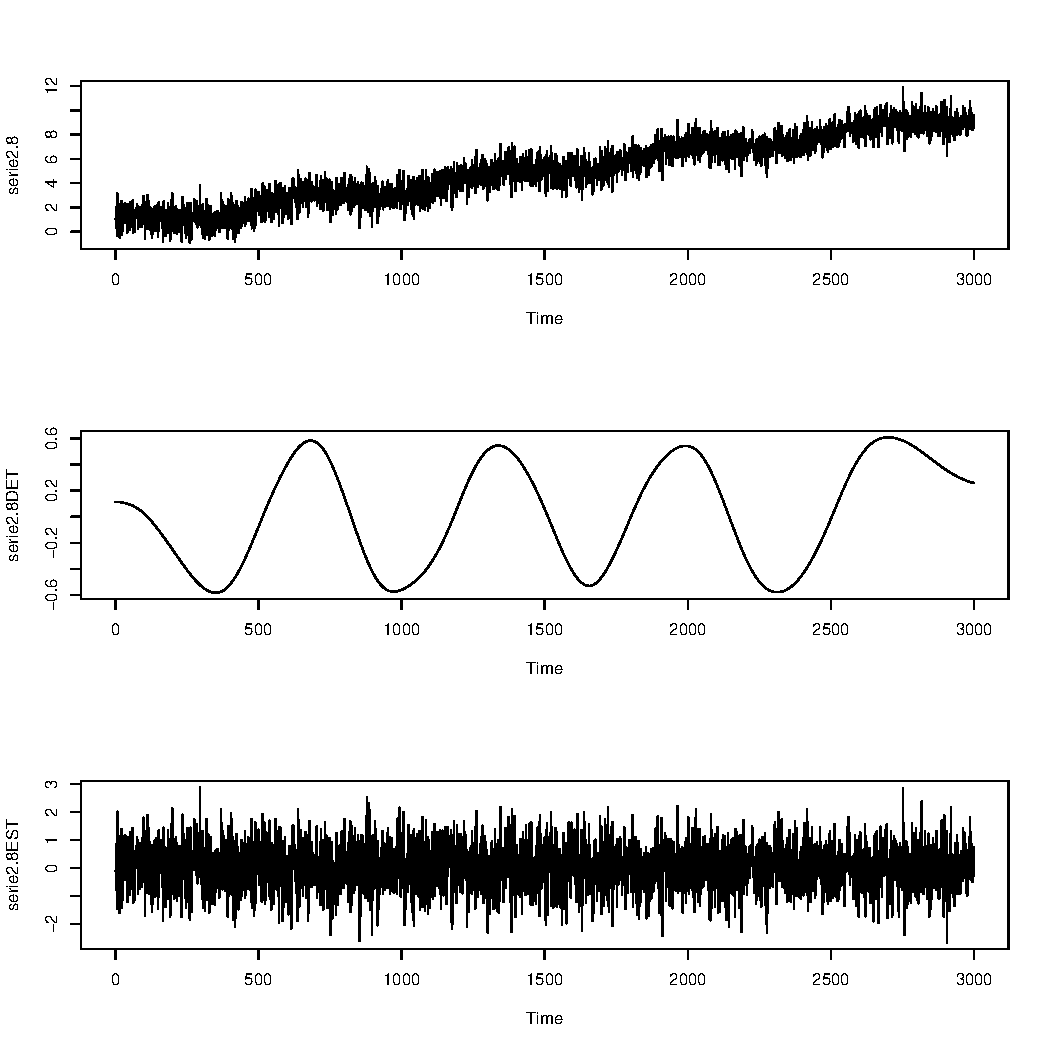
\includegraphics[scale=0.43]{serie2_8.pdf}
  \caption{Série 2.7 e Série 2.8}

\end{center}
\end{figure}

\graphicspath{{imagens/}}
\begin{figure}[H]
\begin{center}
  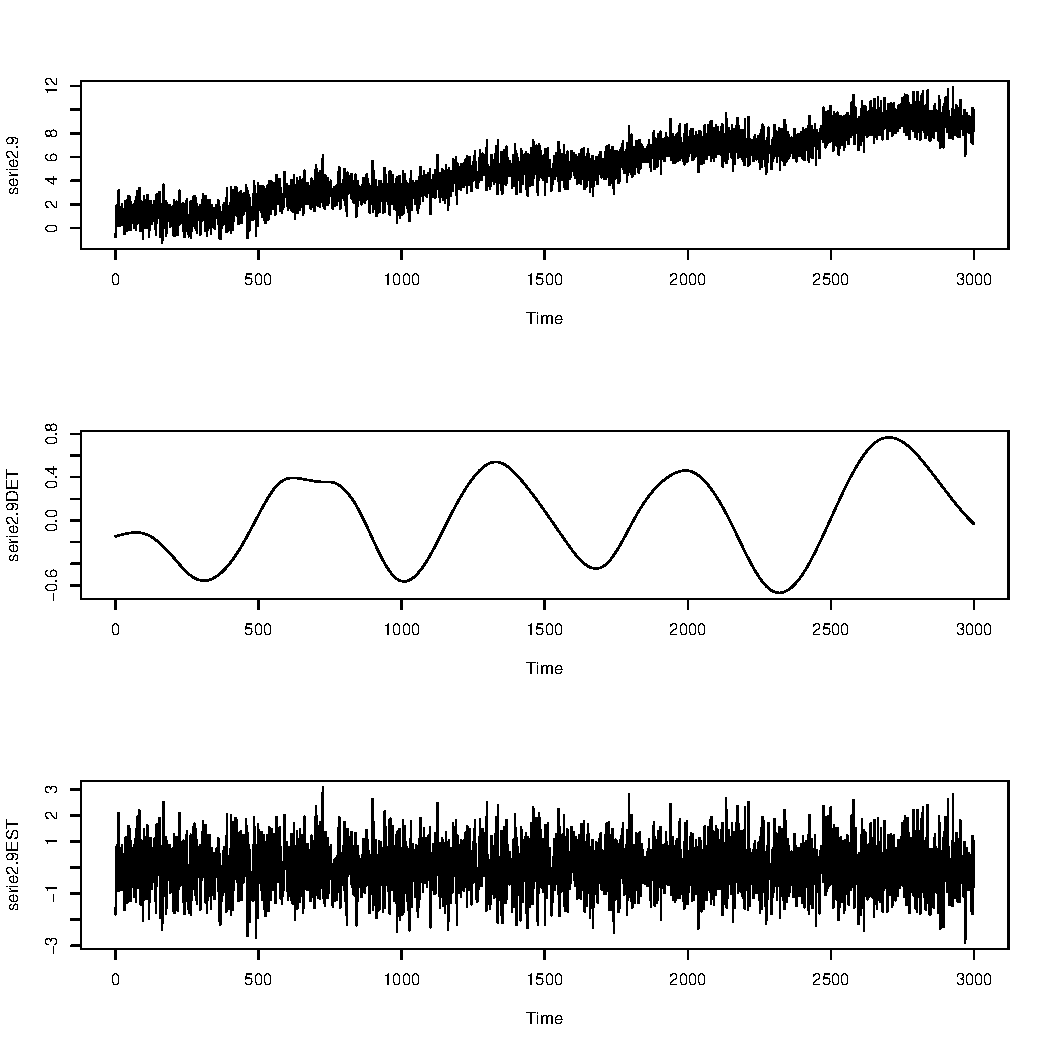
\includegraphics[scale=0.43]{serie2_9.pdf} \quad
  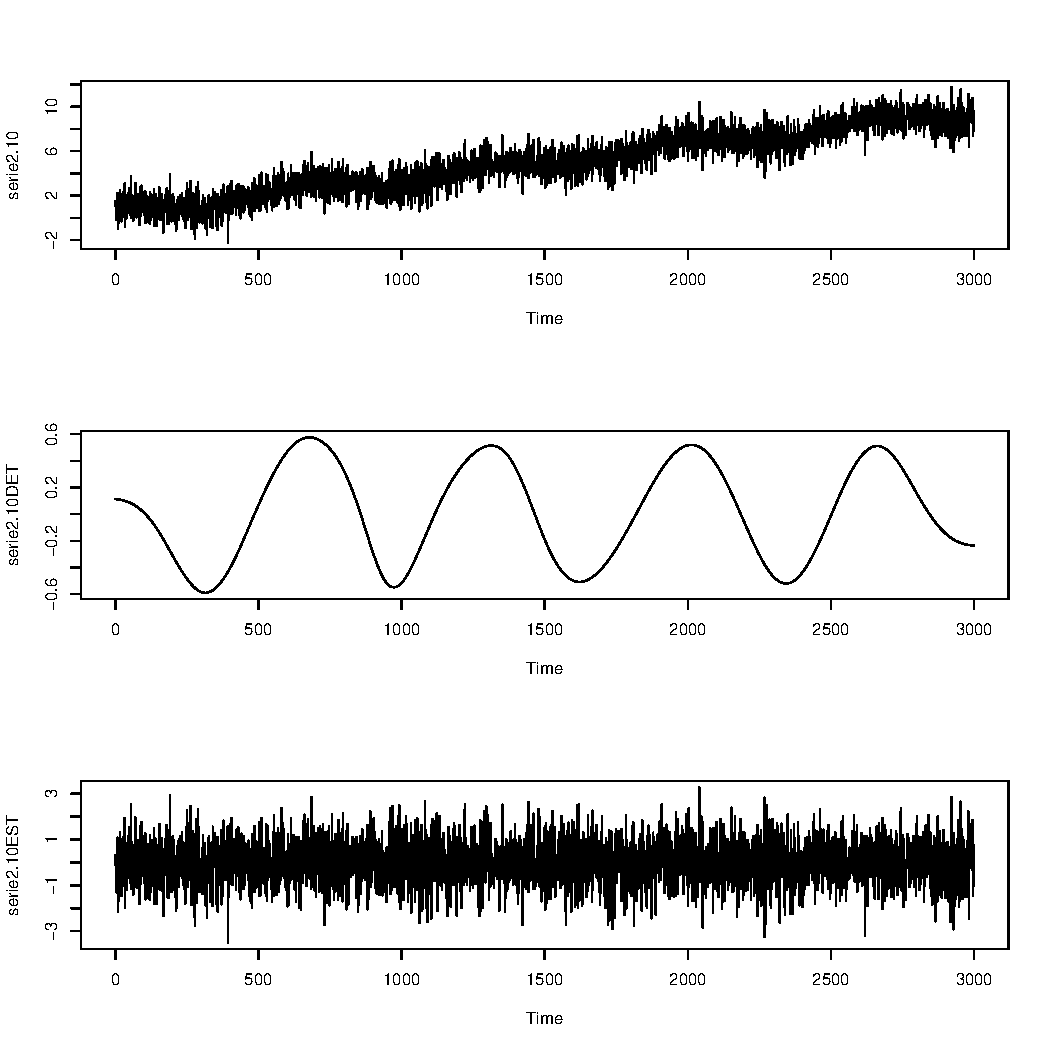
\includegraphics[scale=0.43]{serie2_10.pdf}
  \caption{Série 2.9 e Série 2.10}

\end{center}
\end{figure}

\section{Séries TIPO 3}
10 séries senoide com ruído ao longo da série.
\graphicspath{{imagens/}}
\begin{figure}[H]
\begin{center}
  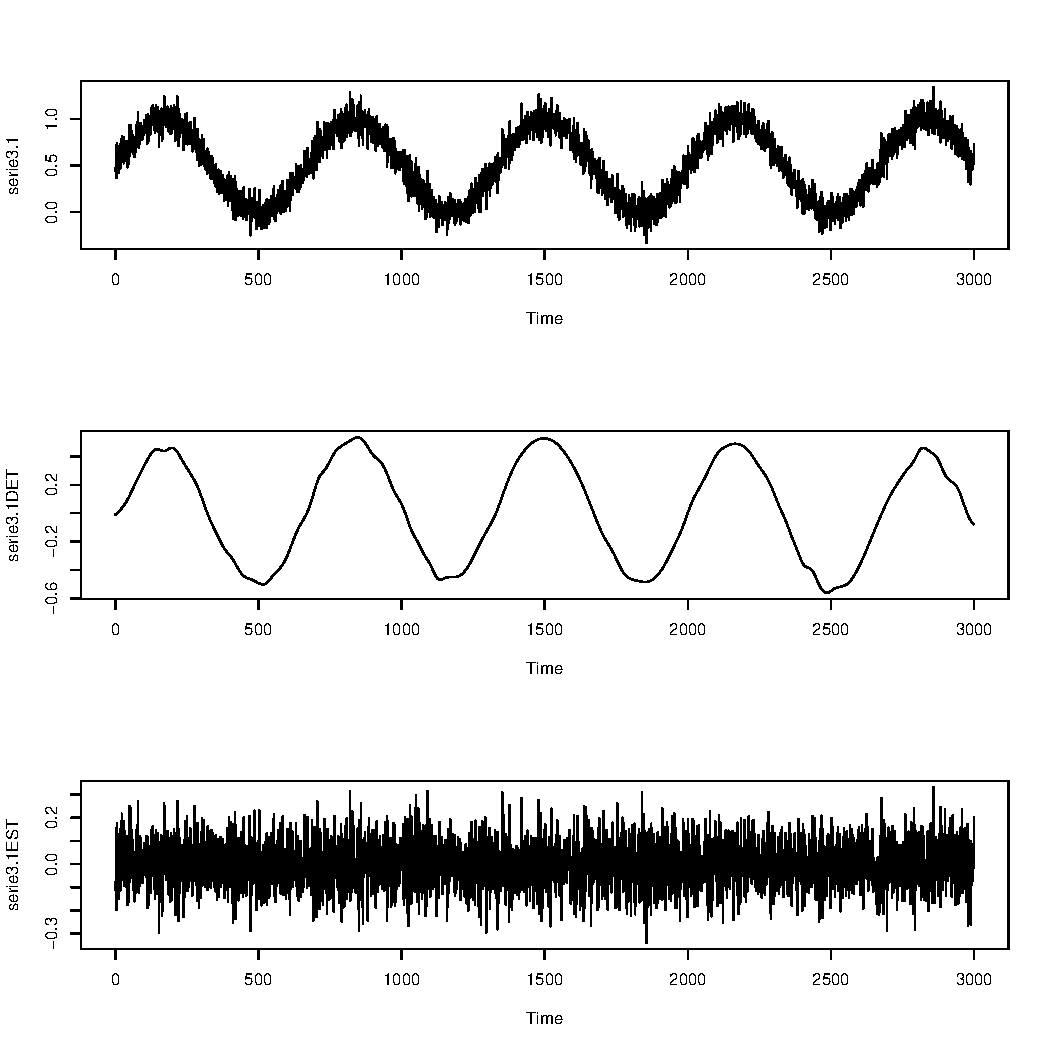
\includegraphics[scale=0.43]{serie3_1.pdf} \quad
  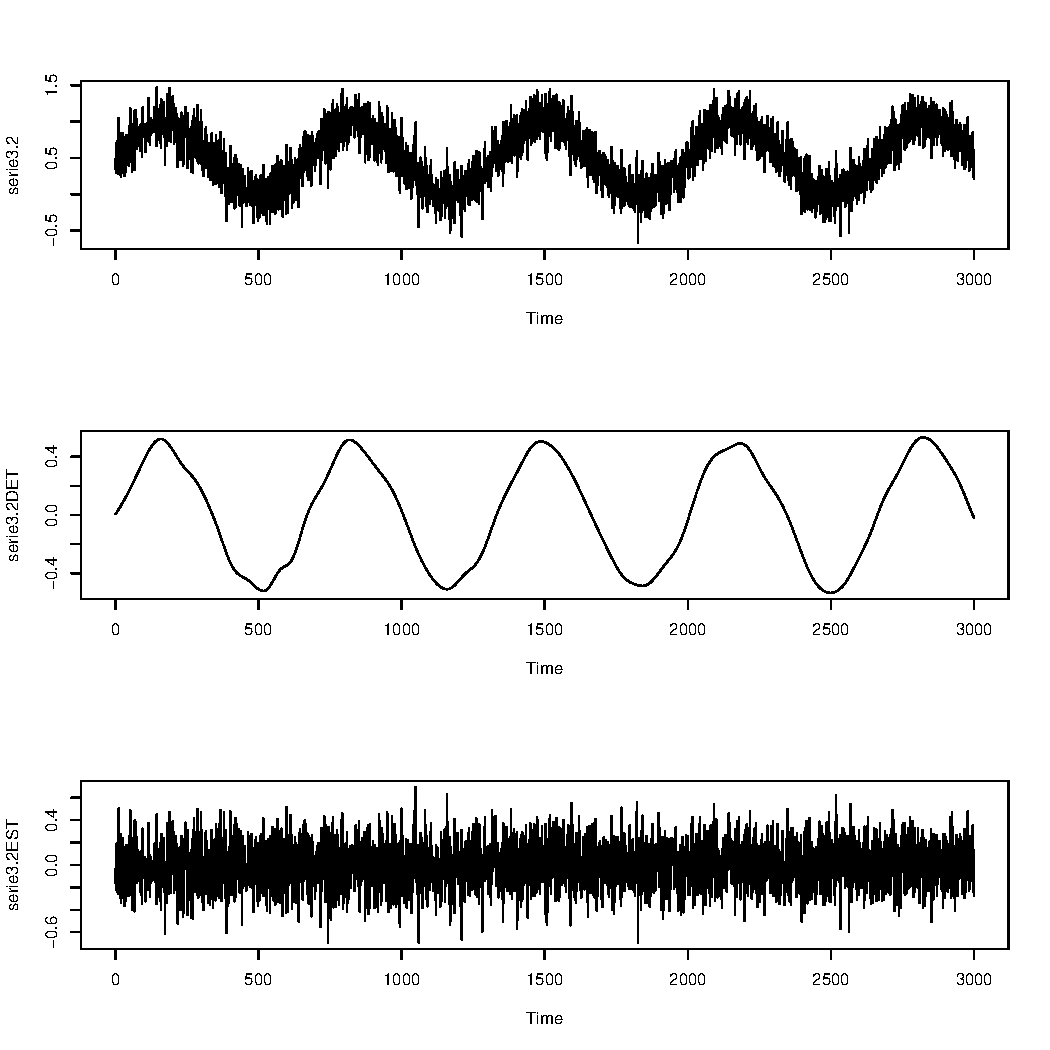
\includegraphics[scale=0.43]{serie3_2.pdf}
  \caption{Série 3.1 e Série 3.2}

\end{center}
\end{figure}

\graphicspath{{imagens/}}
\begin{figure}[H]
\begin{center}
  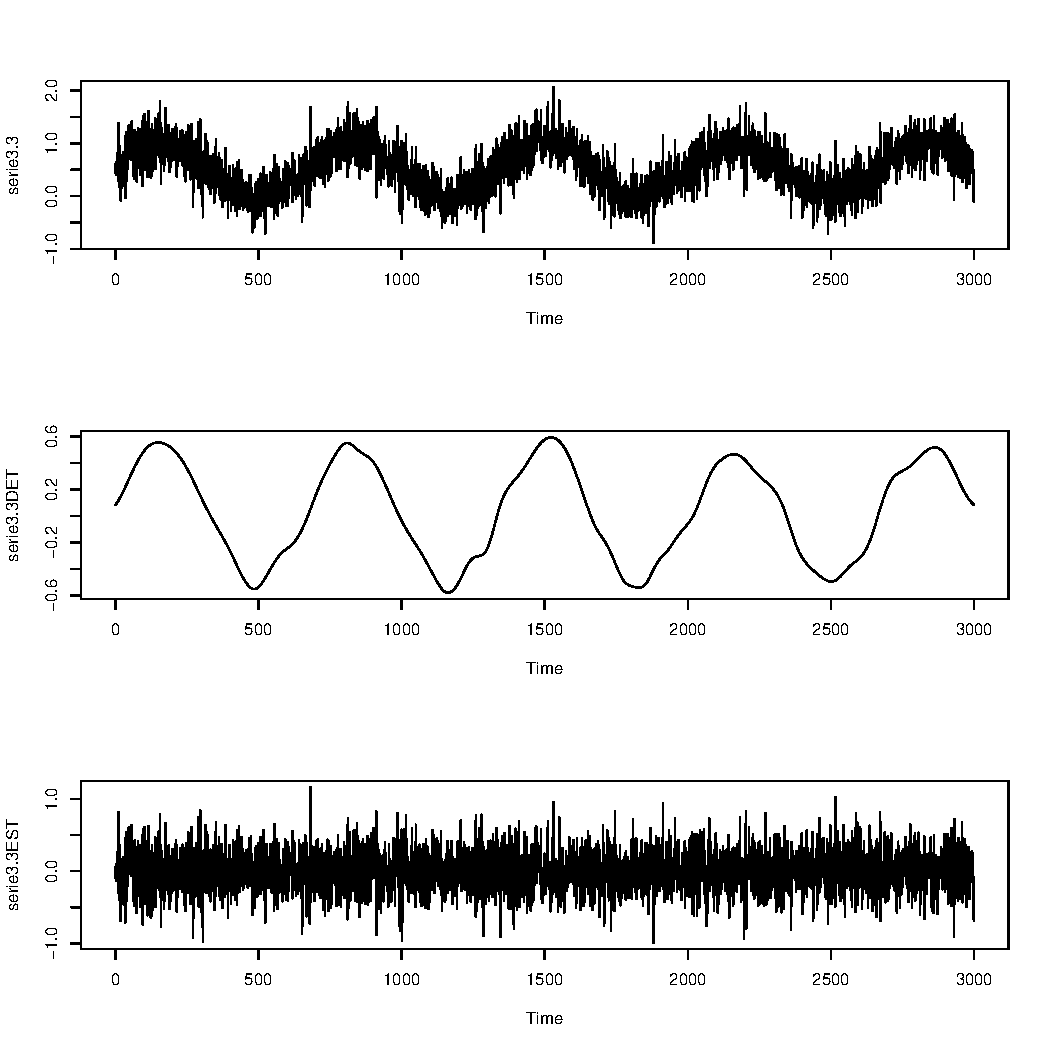
\includegraphics[scale=0.43]{serie3_3.pdf} \quad
  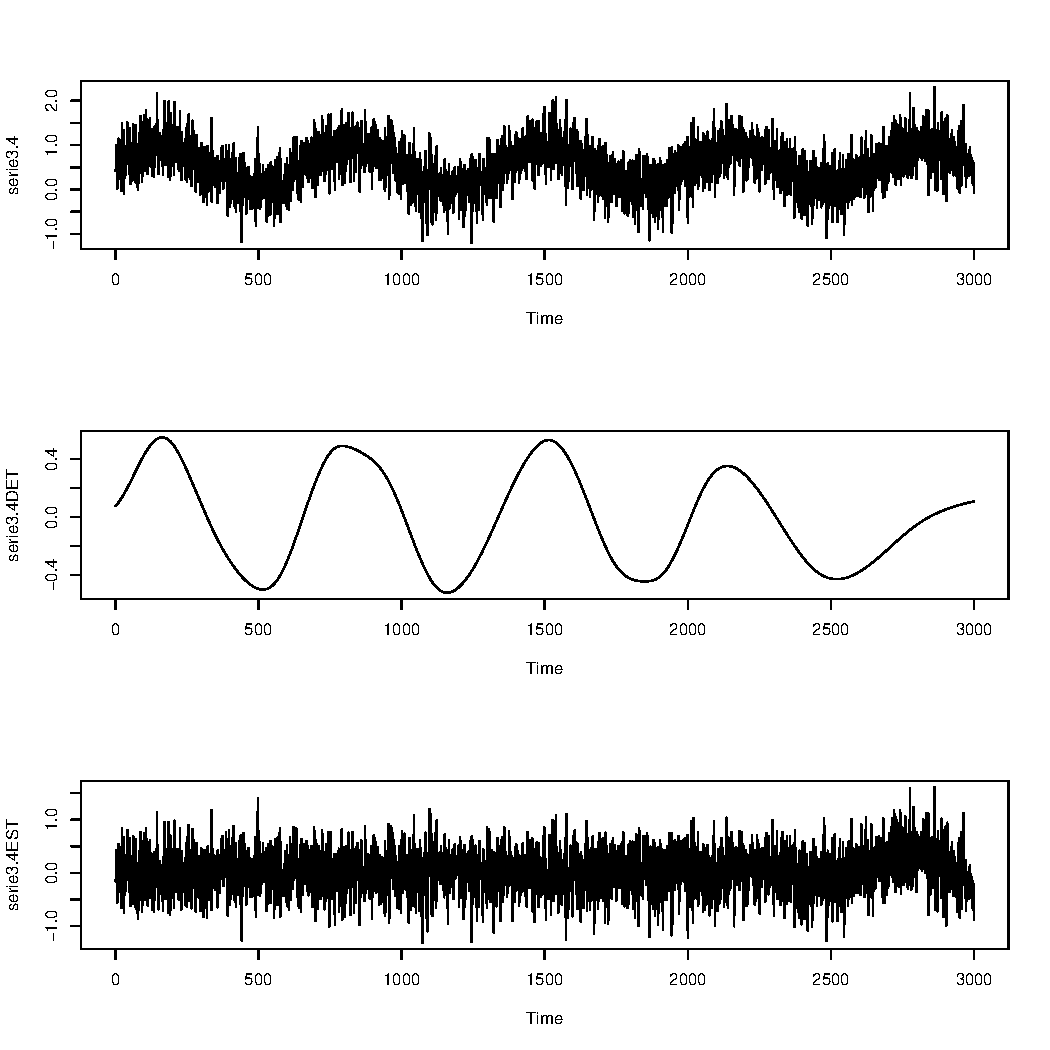
\includegraphics[scale=0.43]{serie3_4.pdf}
  \caption{Série 3.3 e Série 3.4}

\end{center}
\end{figure}

\graphicspath{{imagens/}}
\begin{figure}[H]
\begin{center}
  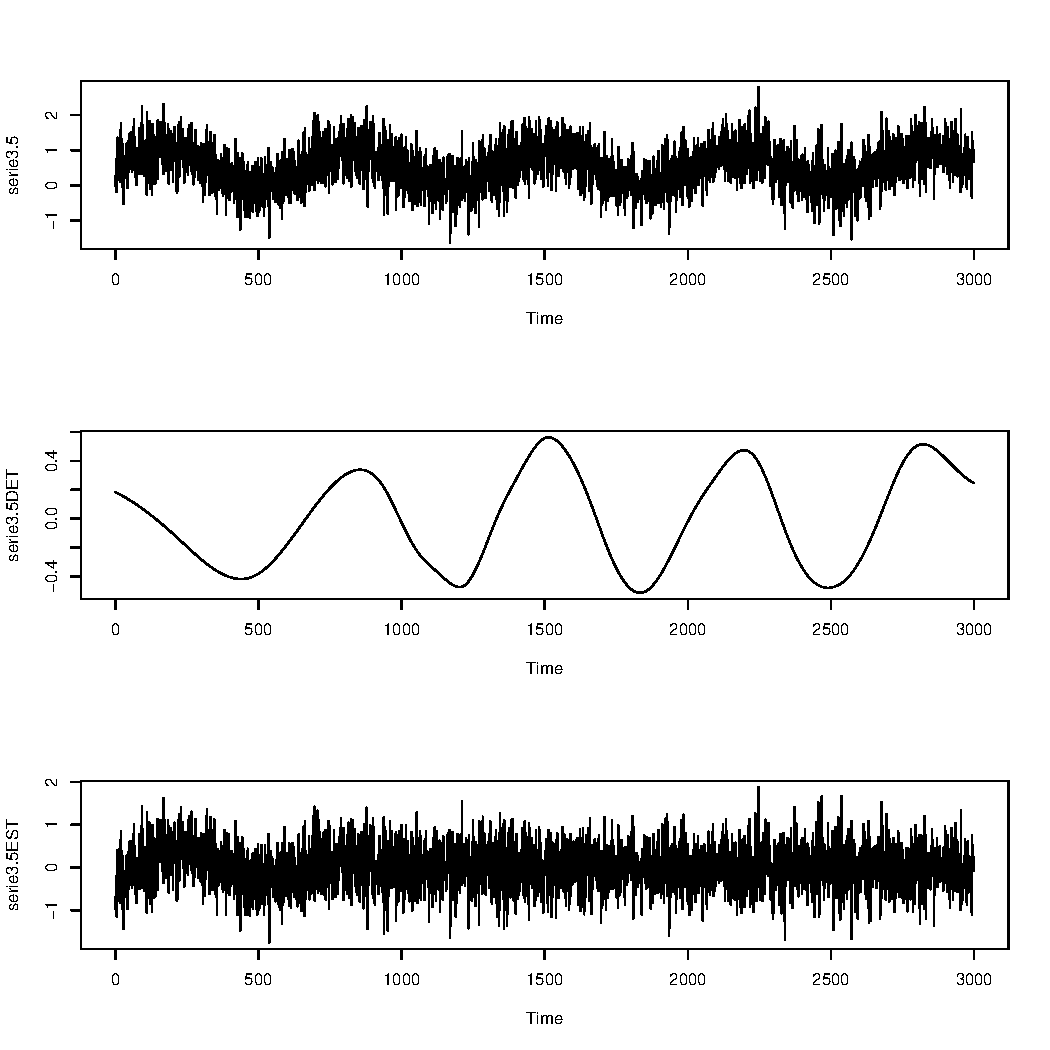
\includegraphics[scale=0.43]{serie3_5.pdf} \quad
  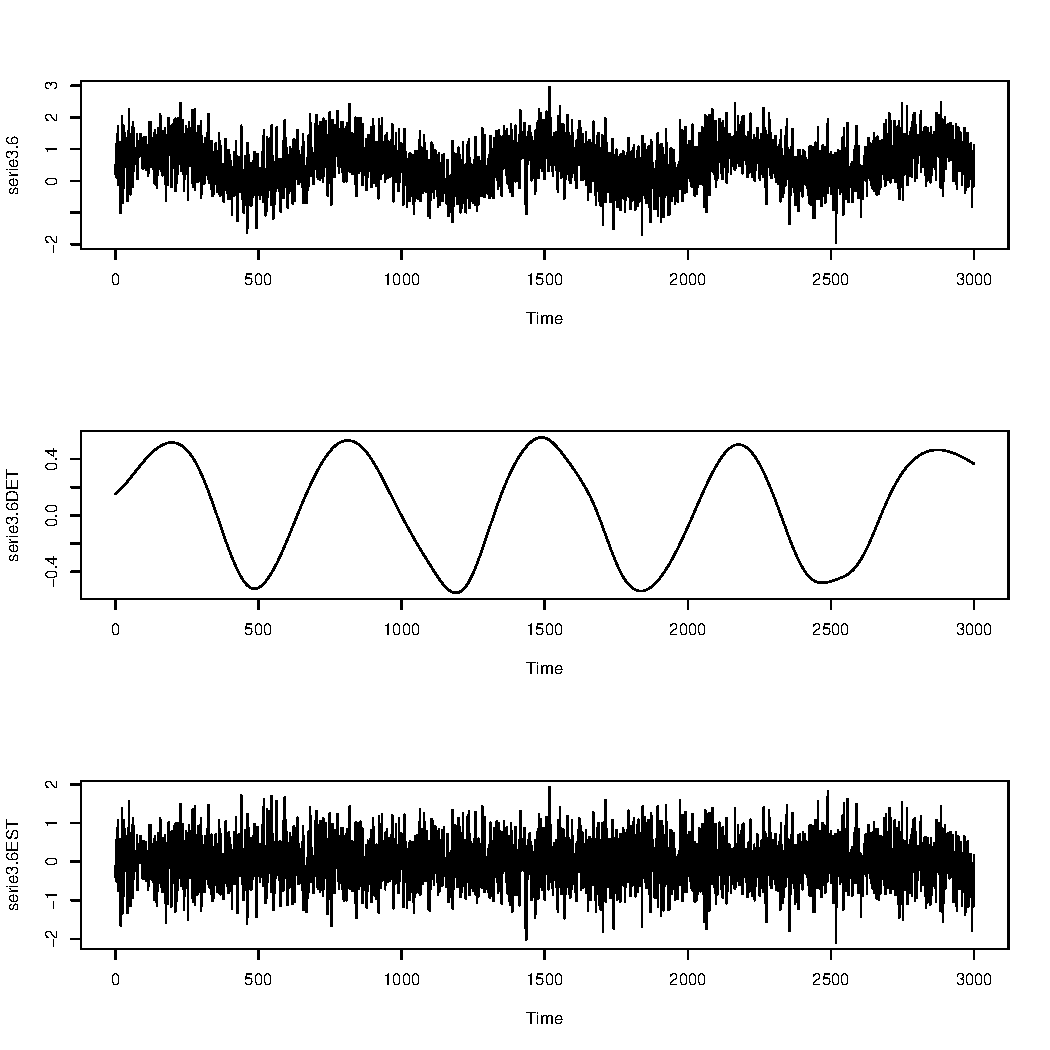
\includegraphics[scale=0.43]{serie3_6.pdf}
  \caption{Série 3.5 e Série 3.6}

\end{center}
\end{figure}

\graphicspath{{imagens/}}
\begin{figure}[H]
\begin{center}
  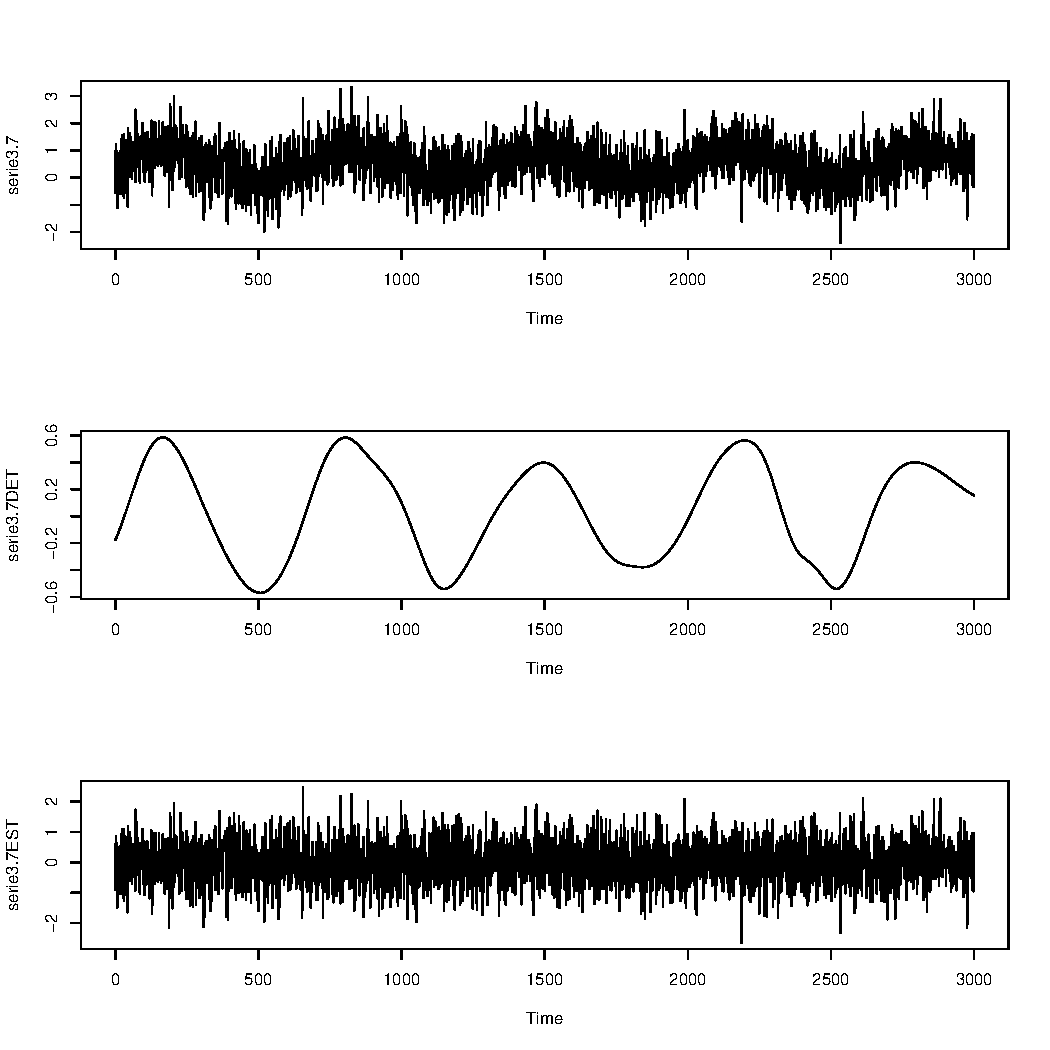
\includegraphics[scale=0.43]{serie3_7.pdf} \quad
  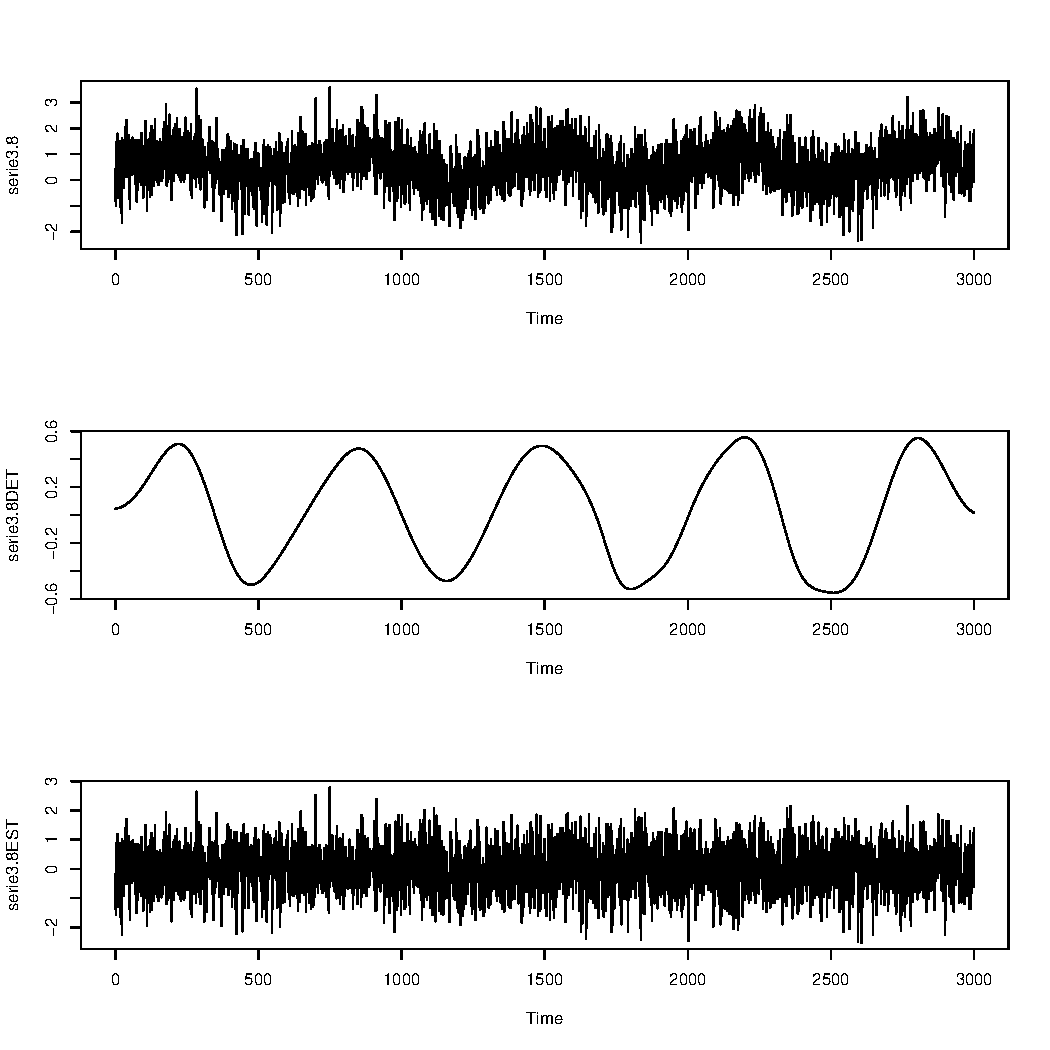
\includegraphics[scale=0.43]{serie3_8.pdf}
  \caption{Série 3.7 e Série 3.8}

\end{center}
\end{figure}

\graphicspath{{imagens/}}
\begin{figure}[H]
\begin{center}
  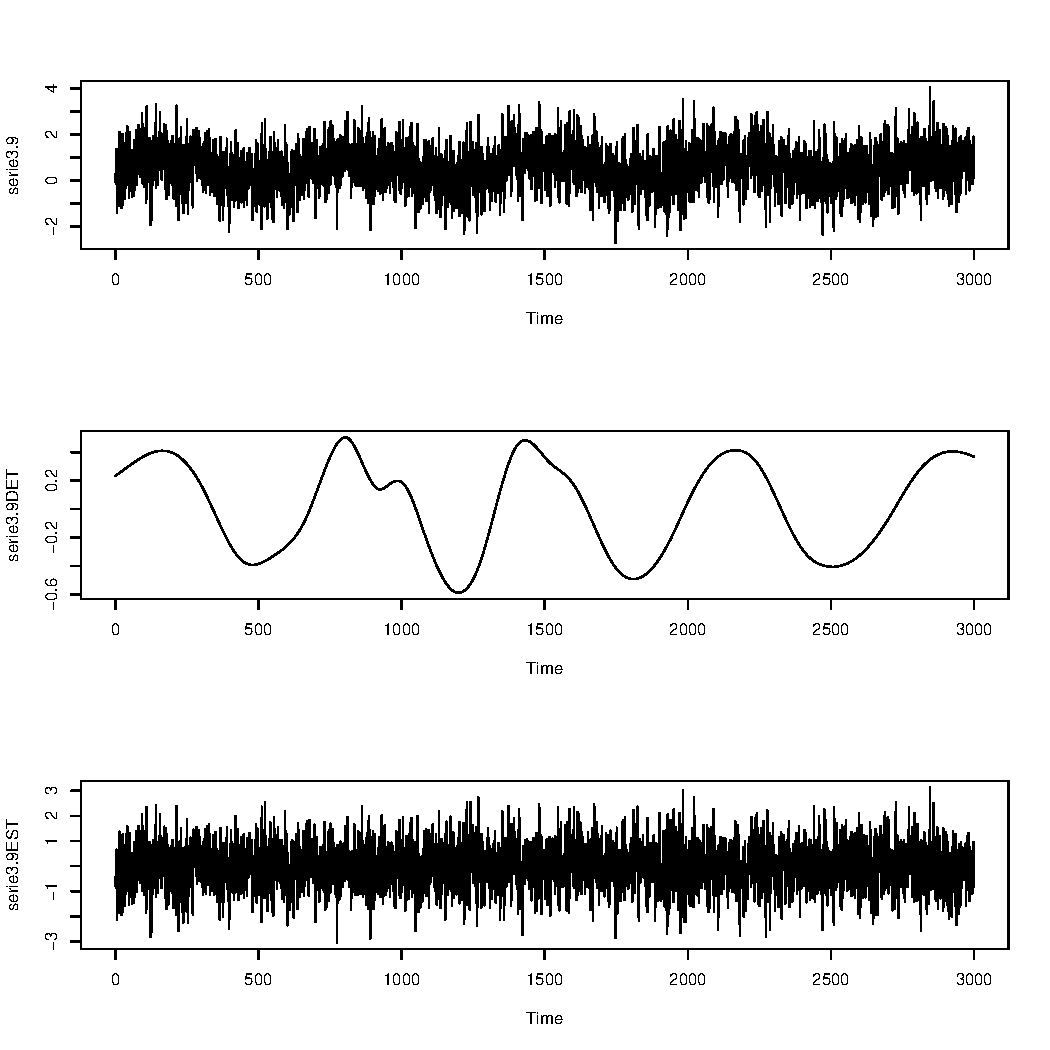
\includegraphics[scale=0.43]{serie3_9.pdf} \quad
  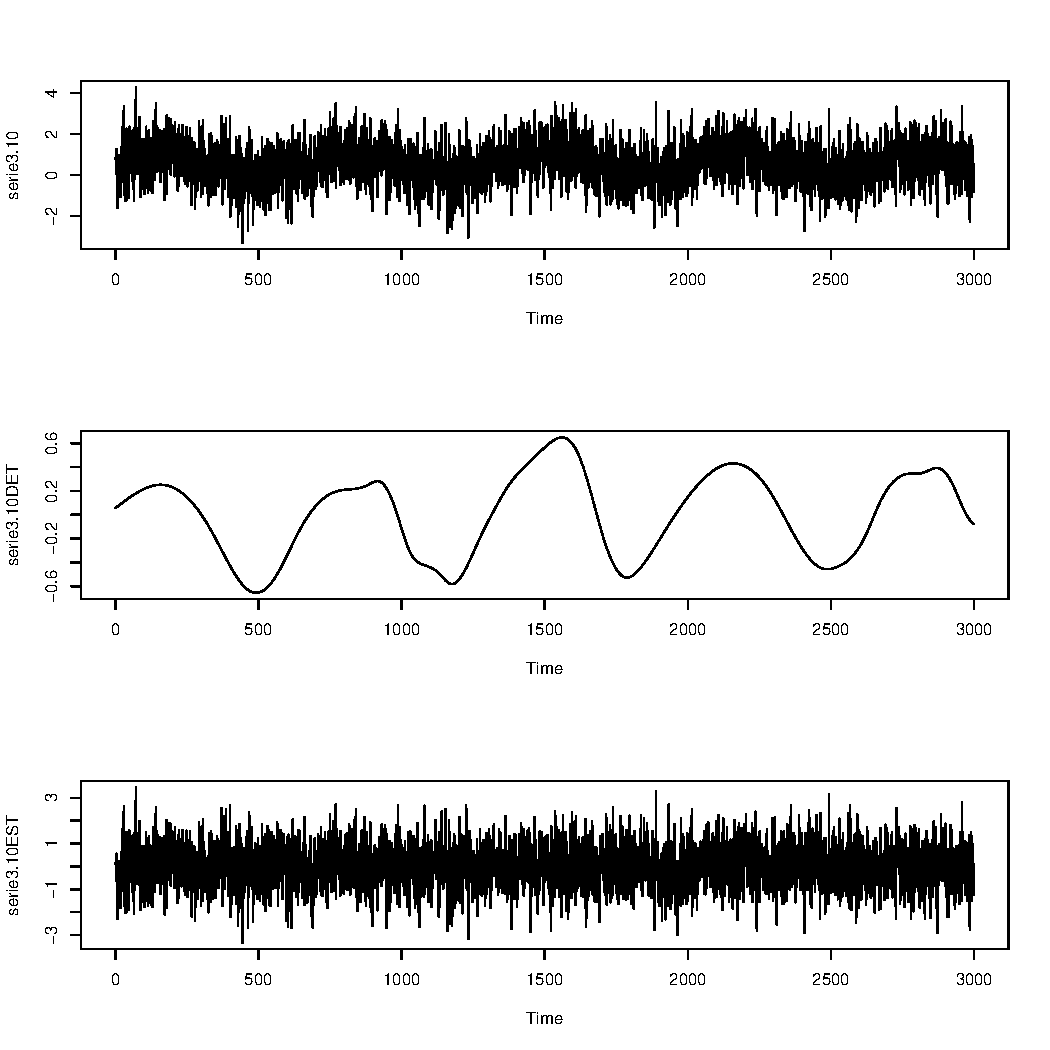
\includegraphics[scale=0.43]{serie3_10.pdf}
  \caption{Série 3.9 e Série 3.10}

\end{center}
\end{figure}

\section{Séries TIPO 4}
10 séries senoide com ruído ao longo da série e tendência.
\graphicspath{{imagens/}}
\begin{figure}[H]
\begin{center}
  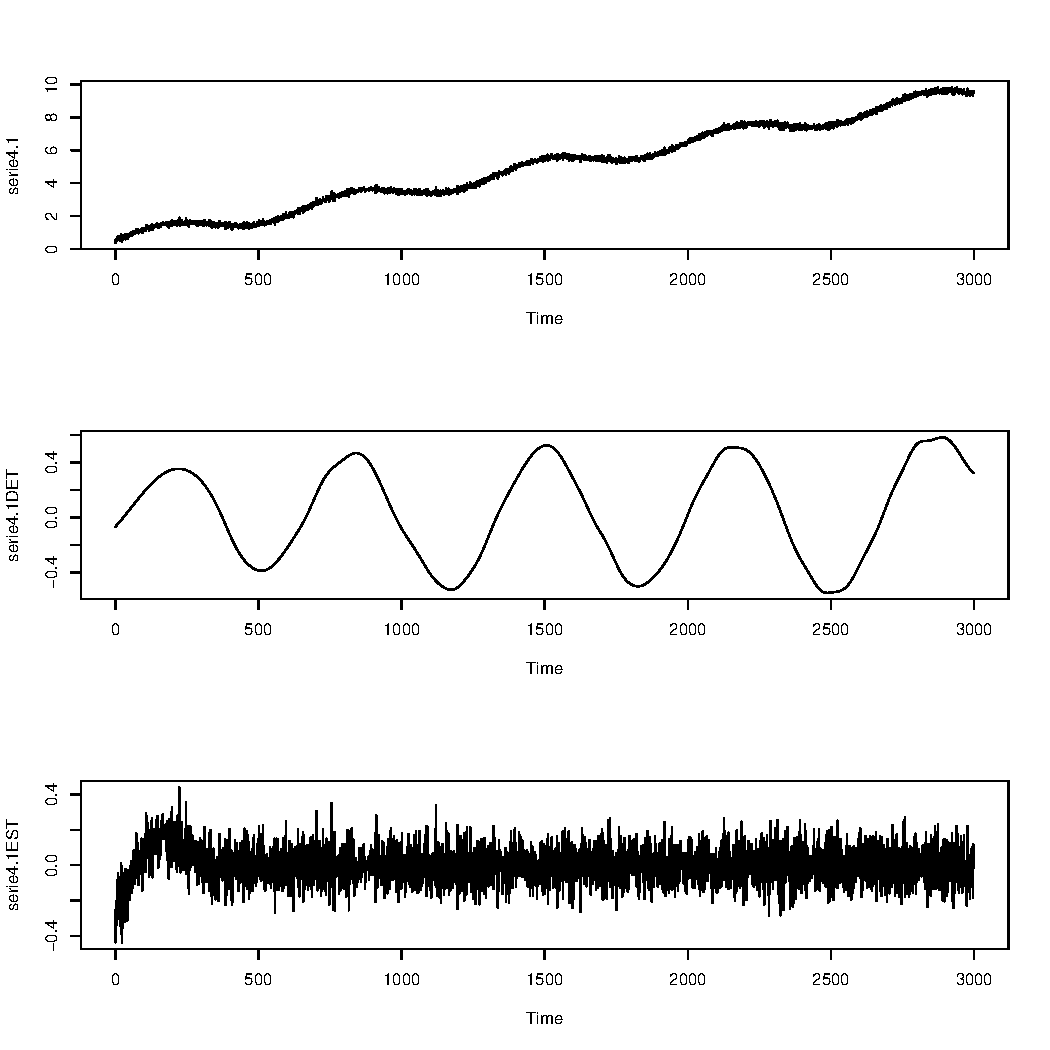
\includegraphics[scale=0.43]{serie4_1.pdf} \quad
  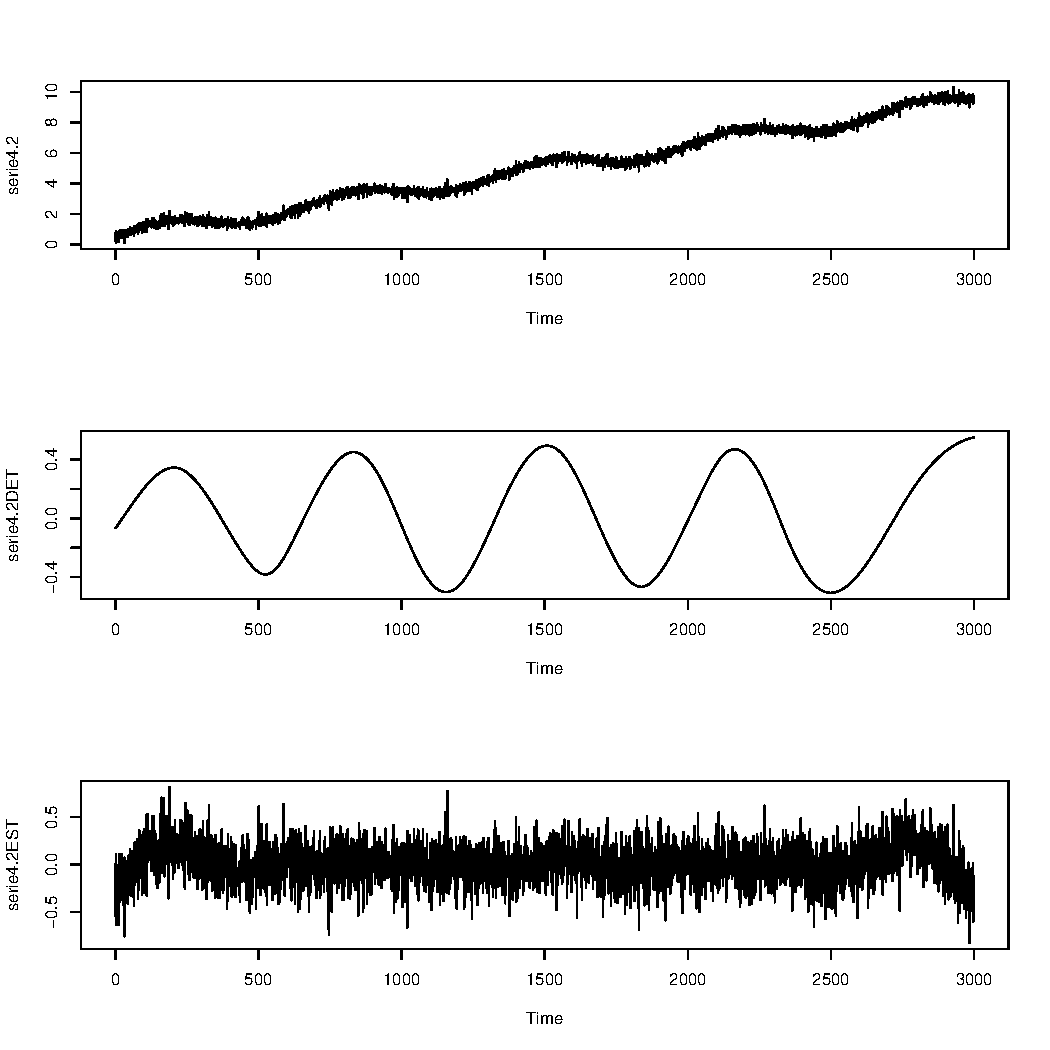
\includegraphics[scale=0.43]{serie4_2.pdf}
  \caption{Série 4.1 e Série 4.2}
\end{center}
\end{figure}

\graphicspath{{imagens/}}
\begin{figure}[H]
\begin{center}
  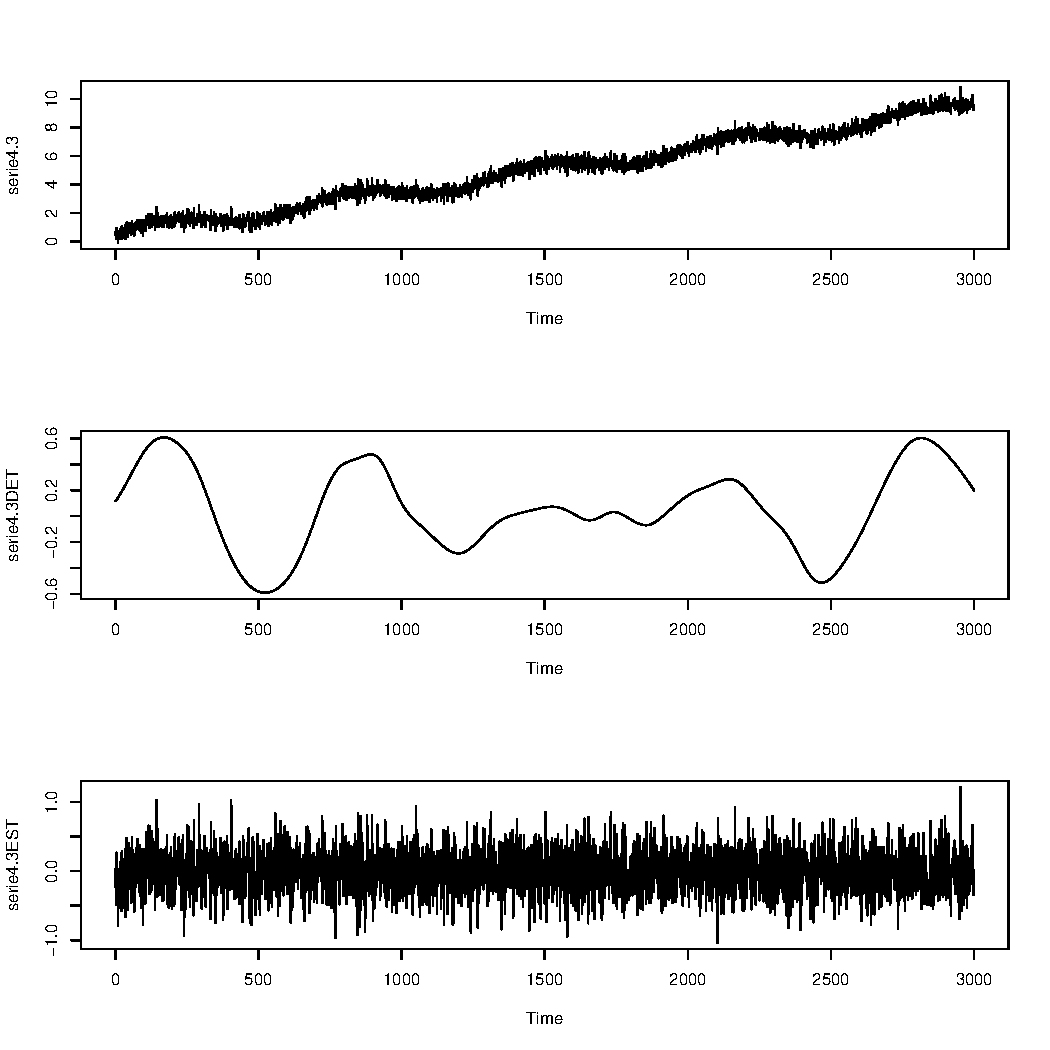
\includegraphics[scale=0.43]{serie4_3.pdf} \quad
 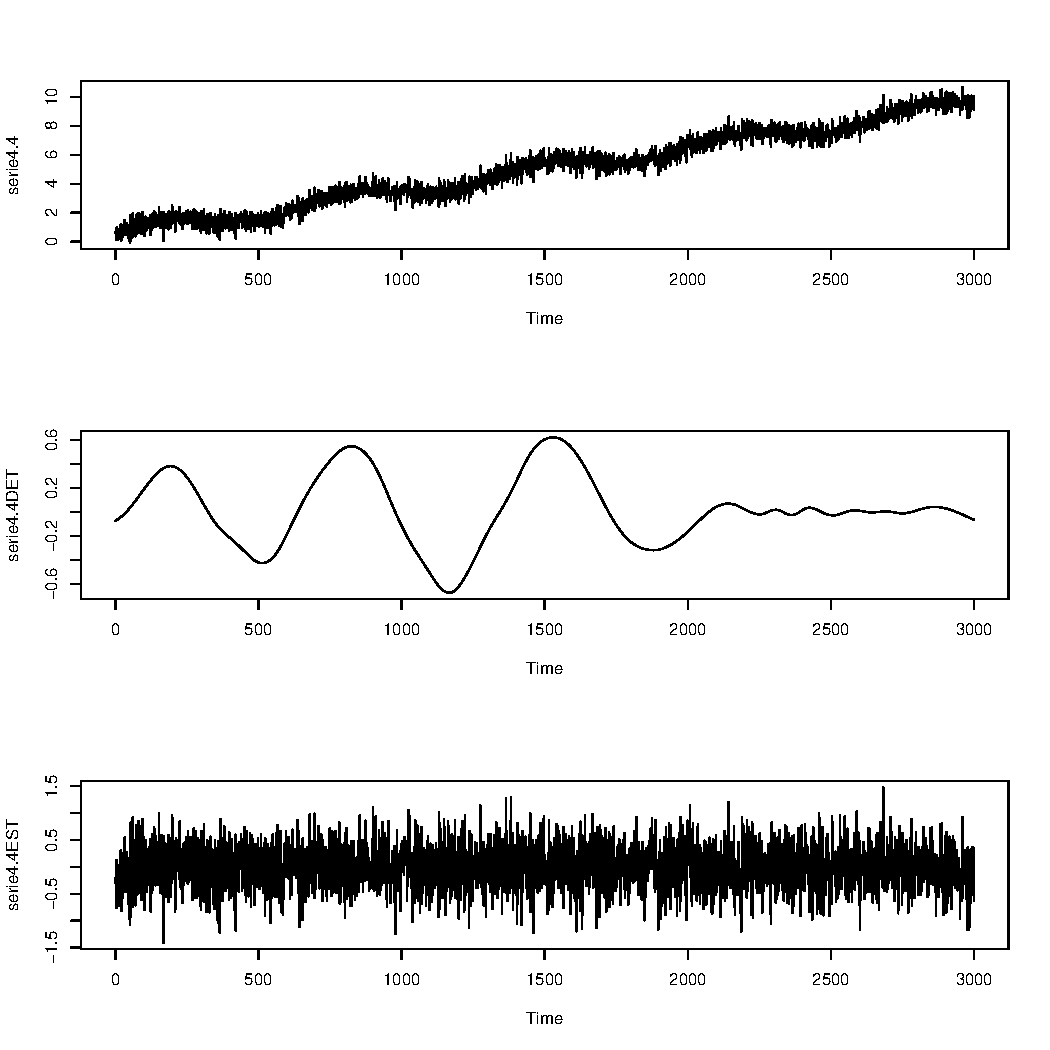
\includegraphics[scale=0.43]{serie4_4.pdf}
 \caption{Série 4.3 e Série 4.4}

\end{center}
\end{figure}

\graphicspath{{imagens/}}
\begin{figure}[H]
\begin{center}
  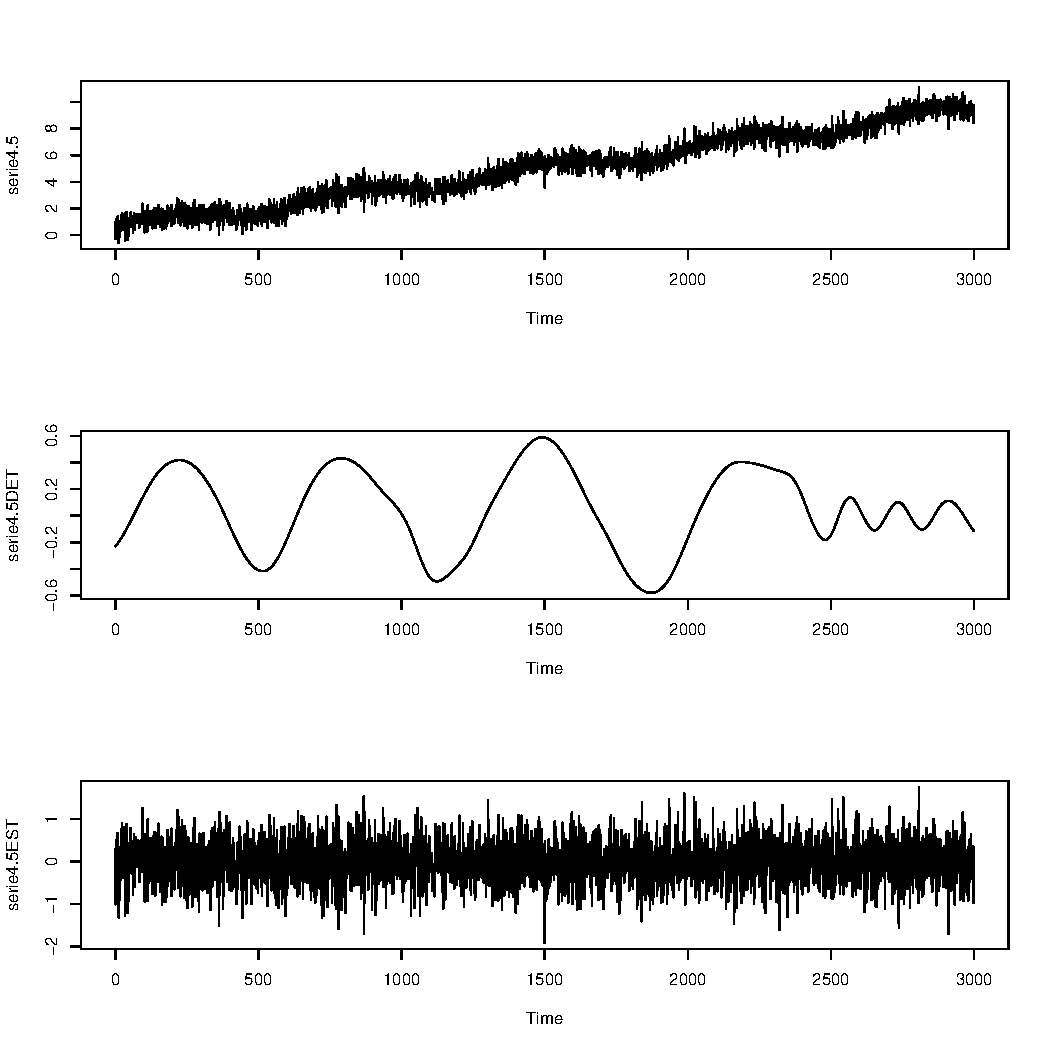
\includegraphics[scale=0.43]{serie4_5.pdf} \quad
  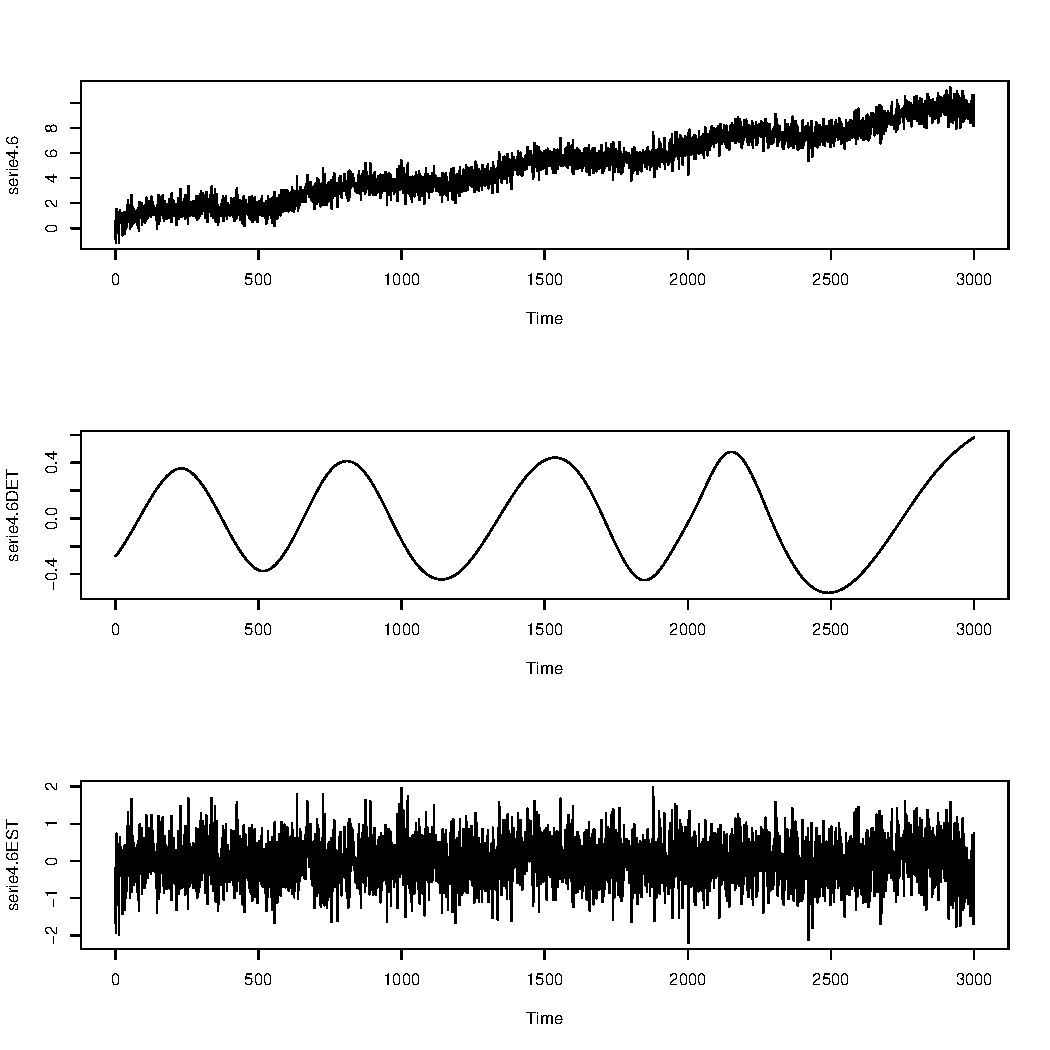
\includegraphics[scale=0.43]{serie4_6.pdf}
 \caption{Série 4.5 e Série 4.6}

\end{center}
\end{figure}

\graphicspath{{imagens/}}
\begin{figure}[H]
\begin{center}
  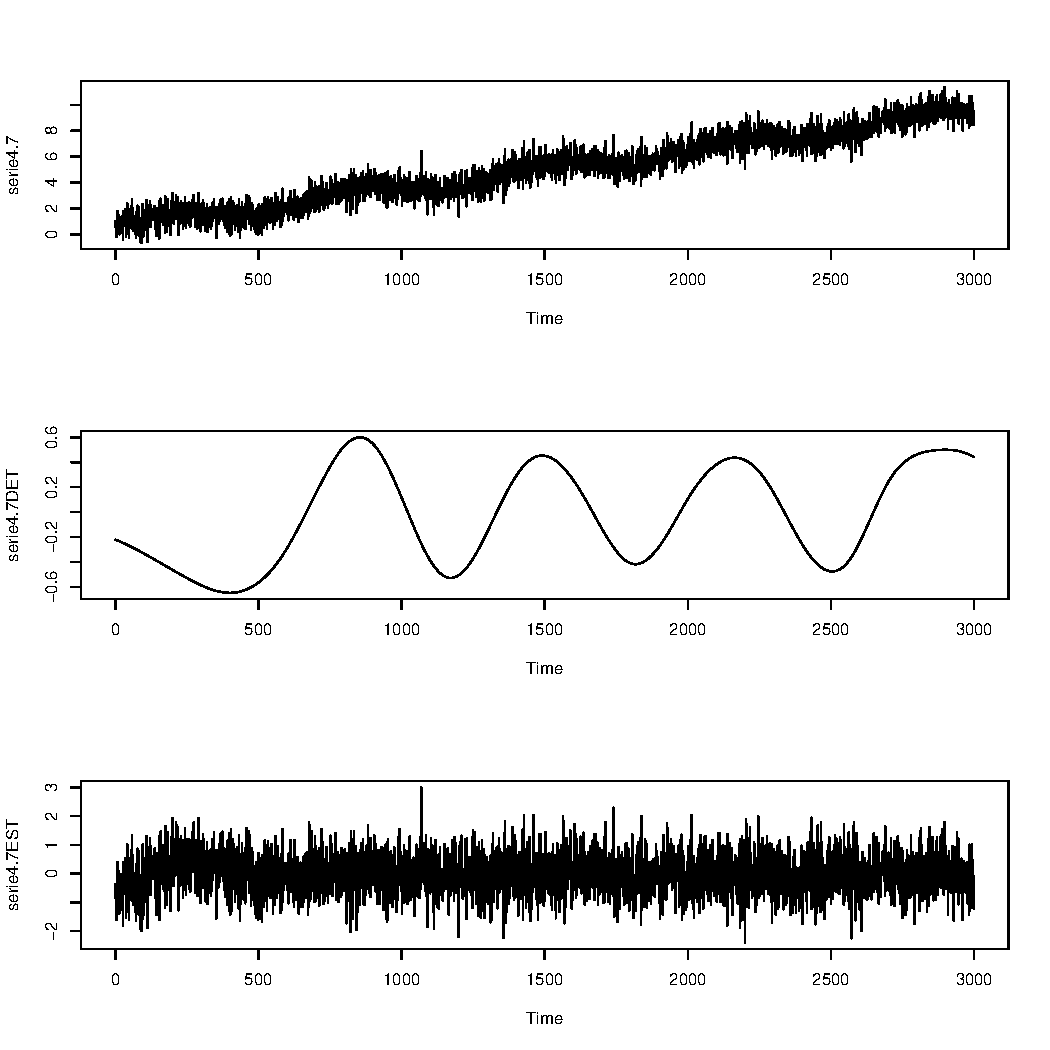
\includegraphics[scale=0.43]{serie4_7.pdf} \quad
  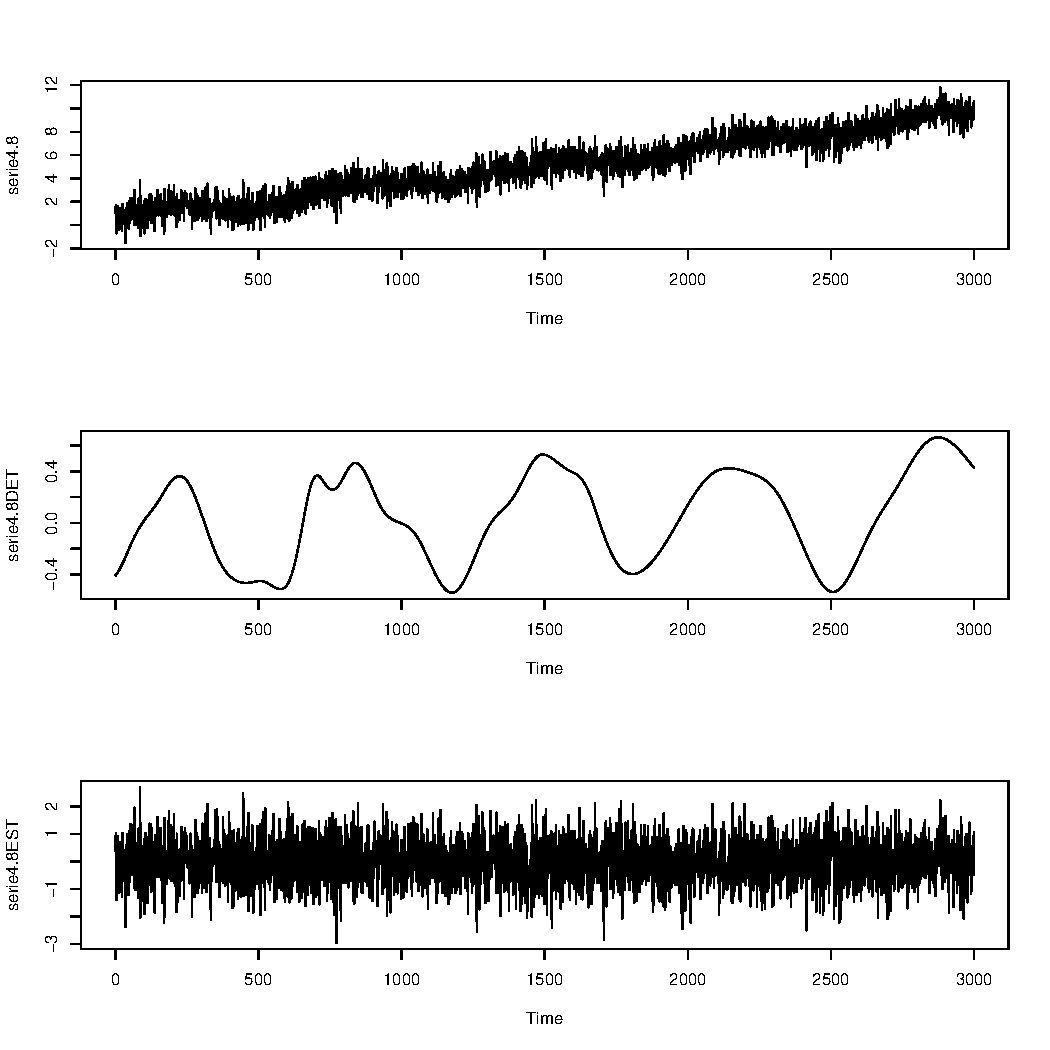
\includegraphics[scale=0.43]{serie4_8.pdf}
  \caption{Série 4.7 e Série 4.8}

\end{center}
\end{figure}

\graphicspath{{imagens/}}
\begin{figure}[H]
\begin{center}
  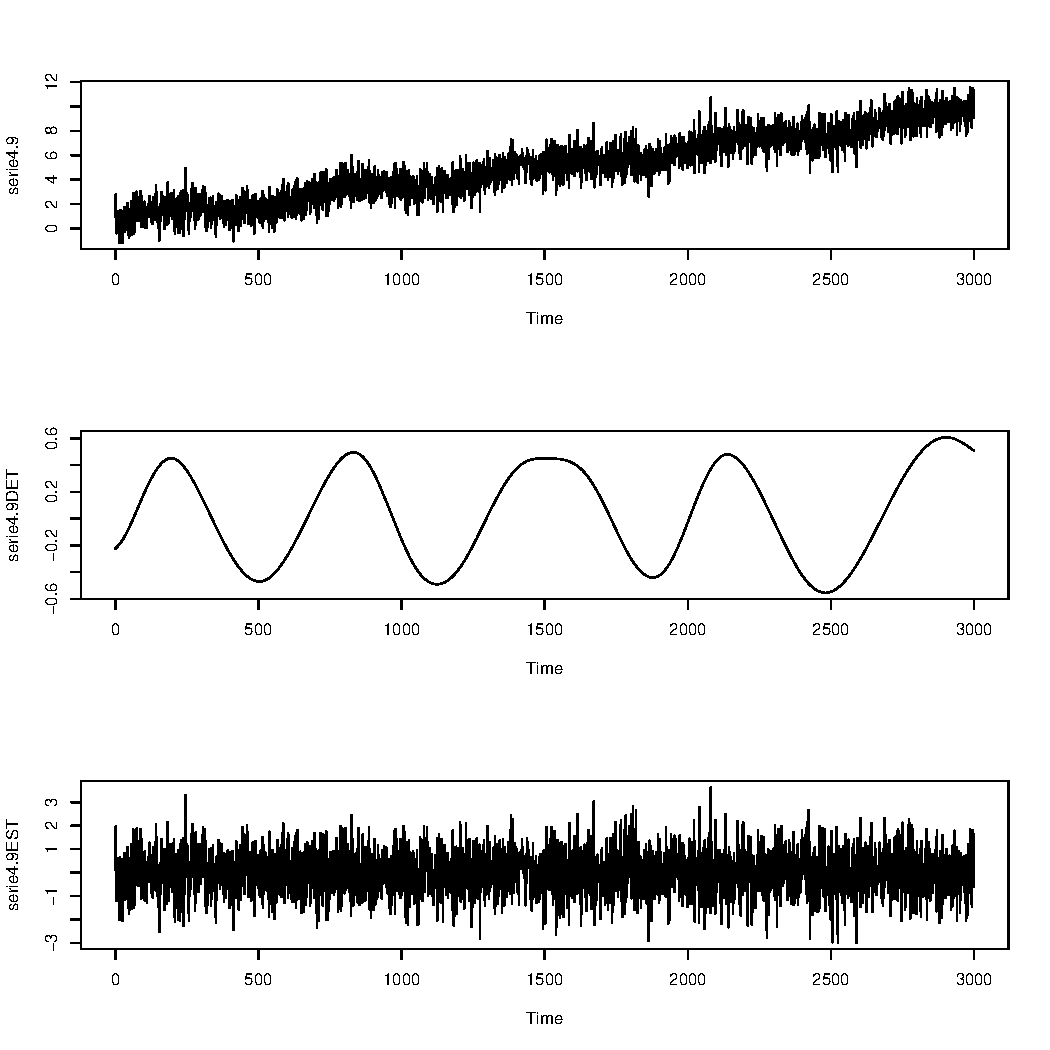
\includegraphics[scale=0.43]{serie4_9.pdf} \quad
  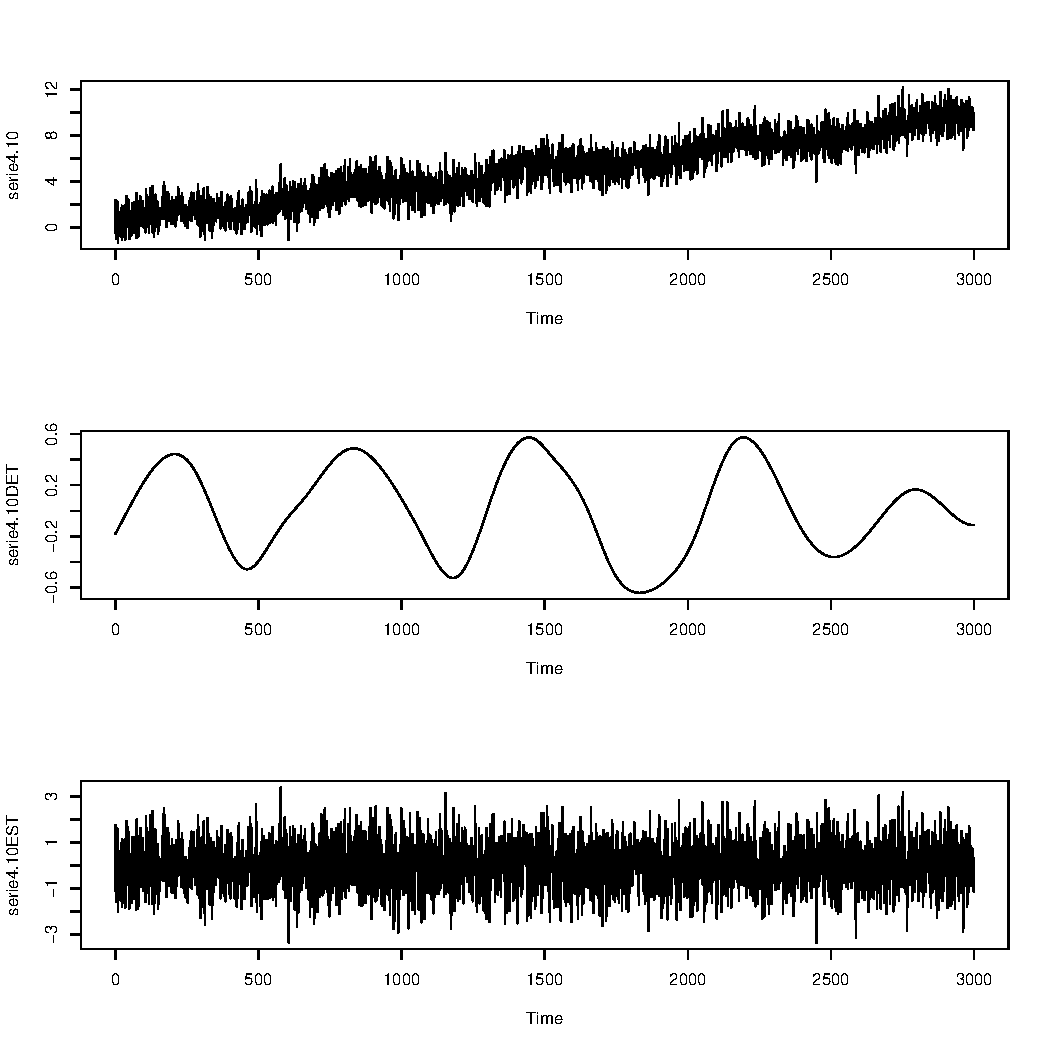
\includegraphics[scale=0.43]{serie4_10.pdf}
  \caption{Série 4.9 e Série 4.10}
\end{center}
\end{figure}
\section{Considerações Finais}
Foram apresentadas as séries temporais utilizadas neste trabalho experimental e suas respactivas decomposições.
% \include{apendice2}
% ...
% \include{apendiceM}

%% Fim do documento
\end{document}
%------------------------------------------------------------------------------------------%
